\documentclass[10pt]{jsarticle}%文字サイズが10ptのjsarticle

%%%%%%%%%%%%%%%%%%%%%%%%%%%%%%%%%%%%%%%%%%%%%%%%%%%%%%%
%%  パッケージ                                        %%
%%%%%%%%%%%%%%%%%%%%%%%%%%%%%%%%%%%%%%%%%%%%%%%%%%%%%%%
%使用しないときはコメントアウトしてください
\usepackage{amsthm}%定理環境
\usepackage{framed}%文章を箱で囲う
\usepackage{amsmath,amssymb}%数式全般
\usepackage[dvipdfmx]{graphicx}%図の挿入
%\usepackage{tikz}%描画
\usepackage{titlesec}%見出しの見た目を編集できる
\usepackage[dvipdfmx, usenames]{color}%色をつける
%\usepackage{tikz-cd}%可換図式
%\usepackage{mathtools}%数式関連
\usepackage{amsfonts}%数式のフォント
\usepackage[all]{xy}%可換図式
\usepackage{mathrsfs}%花文字
\usepackage{comment}%コメント環境
\usepackage{picture}%お絵かき
\usepackage{url}%URLを出力
\usepackage[dvipdfmx]{hyperref}
\usepackage{pxjahyper}%日本語しおりの文字化けを防ぐ

%%%%%%%%%%%%%%%%%%%%%%%%%%%%%%%%%%%%%%%%%%%%%%%%%%%%%%%
%%  表紙                                             %%
%%%%%%%%%%%%%%%%%%%%%%%%%%%%%%%%%%%%%%%%%%%%%%%%%%%%%%%
\makeatletter
\def\thickhrulefill{\leavevmode \leaders \hrule height 1pt\hfill \kern \z@}
\renewcommand{\maketitle}{\begin{titlepage}%
    \let\footnotesize\small
    \let\footnoterule\relax
    \parindent \z@
    \reset@font
    \null\vfil
    \begin{flushleft}
      \huge \@title
    \end{flushleft}
    \par
    \hrule height 4pt
    \par
    \begin{flushright}
      \LARGE \@author \par
    \end{flushright}
    \vskip 60\p@
    \vfil\null
    \begin{flushright}
        {\small \@date}%
    \end{flushright}
  \end{titlepage}%
  \setcounter{footnote}{0}%
}
\makeatother

%%%%%%%%%%%%%%%%%%%%%%%%%%%%%%%%%%%%%%%%%%%%%%%%%%%%%%%
%%  sectionの修飾                                     %%
%%%%%%%%%%%%%%%%%%%%%%%%%%%%%%%%%%%%%%%%%%%%%%%%%%%%%%%
\titleformat{\section}[block]
{}{}{0pt}
{
  \colorbox{black}{\begin{picture}(0,10)\end{picture}}
  \hspace{0pt}
  \normalfont \Large\bfseries
  \hspace{-4pt}
}
[
\begin{picture}(100,0)
  \put(3,18){\color{black}\line(1,0){300}}
\end{picture}
\\
\vspace{-30pt}
]

%%%%%%%%%%%%%%%%%%%%%%%%%%%%%%%%%%%%%%%%%%%%%%%%%%%%%%%
%%  太字section                                     %%
%%%%%%%%%%%%%%%%%%%%%%%%%%%%%%%%%%%%%%%%%%%%%%%%%%%%%%%
\newcommand{\bfsubsection}[1]{\subsection*{\textbf{#1}}}
\newcommand{\bfsection}[1]{\section*{\textbf{#1}}}

%%%%%%%%%%%%%%%%%%%%%%%%%%%%%%%%%%%%%%%%%%%%%%%%%%%%%%%
%%  番号付き定理環境                                  %%
%%%%%%%%%%%%%%%%%%%%%%%%%%%%%%%%%%%%%%%%%%%%%%%%%%%%%%%
%注:defというコマンドはもうある
\theoremstyle{definition}%定理環境のアルファベットを斜体にしない
\renewcommand{\proofname}{\textgt{証明}}%proof環境の修正

%%%%%%%%%%%%%%%%%%%%%%%%%%%%%%%%%%%%%%%%%%%%%%%%%%%%%%%
%%  番号なし定理環境                                  %%
%%%%%%%%%%%%%%%%%%%%%%%%%%%%%%%%%%%%%%%%%%%%%%%%%%%%%%%
%一部箱付き
\newtheorem*{lemma}{補題}
\newtheorem*{proposition}{命題}
\newtheorem*{definition}{定義}
\newcommand{\lem}[1]{\begin{oframed} \begin{lemma} #1 \end{lemma} \end{oframed}}%箱付きほだい
\newcommand{\prop}[1]{\begin{oframed} \begin{proposition} #1 \end{proposition} \end{oframed}}%箱付きめいだい

\newtheorem*{claim}{主張}
\newtheorem*{sol}{解答}
\newtheorem*{prob}{問題}
\newtheorem*{quo}{引用}
\newtheorem*{rem}{注意}



%%%%%%%%%%%%%%%%%%%%%%%%%%%%%%%%%%%%%%%%%%%%%%%%%%%%%%%
%%  左側に線を引く                                  %%
%%%%%%%%%%%%%%%%%%%%%%%%%%%%%%%%%%%%%%%%%%%%%%%%%%%%%%%
%leftbar環境の定義
\makeatletter
\renewenvironment{leftbar}{%
%  \def\FrameCommand{\vrule width 3pt \hspace{10pt}}%  デフォルトの線の太さは3pt
  \renewcommand\FrameCommand{\vrule width 1pt \hspace{10pt}}%
  \MakeFramed {\advance\hsize-\width \FrameRestore}}%
 {\endMakeFramed}
\newcommand{\exbf}[2]{ \begin{leftbar} \textbf{#1} #2 \end{leftbar} }%左線つき太字
%\newcommand{\barquo}[1]{\begin{leftbar} \begin{quo} #1 \end{quo} \end{leftbar}}%左線つき引用%びふぉあ
\newcommand{\barquo}[1]{\begin{leftbar} \noindent #1  \end{leftbar}}%左線つき引用%あふたー
\newcommand{\lbar}[1]{\begin{leftbar} #1 \end{leftbar}}



%%%%%%%%%%%%%%%%%%%%%%%%%%%%%%%%%%%%%%%%%%%%%%%%%%%%%%%
%%  色をつける                                      %%
%%%%%%%%%%%%%%%%%%%%%%%%%%%%%%%%%%%%%%%%%%%%%%%%%%%%%%%
\newcommand{\textblue}[1]{\textcolor{blue}{\textbf{#1}}}

%%%%%%%%%%%%%%%%%%%%%%%%%%%%%%%%%%%%%%%%%%%%%%%%%%%%%%%
%%  よく使う記号の略記                                 %%
%%%%%%%%%%%%%%%%%%%%%%%%%%%%%%%%%%%%%%%%%%%%%%%%%%%%%%%
\newcommand{\setmid}[2]{\left\{ #1 \mathrel{} \middle| \mathrel{} #2 \right\}}%集合の内包記法
\newcommand{\sm}{\setminus}%集合差
\newcommand{\abs}[1]{\left \lvert #1 \right \rvert}%絶対値
\newcommand{\norm}[1]{\left \lVert #1 \right \rVert}%ノルム
\newcommand{\transpose}[1]{\, {\vphantom{#1}}^t\!{#1}}%行列の転置
\newcommand{\pmat}[1]{ \begin{pmatrix} #1 \end{pmatrix} }%まるかっこ行列
\newcommand{\f}[2]{\frac{#1}{#2}}%分数
\newcommand{\kakko}[1]{ \langle #1  \rangle}%鋭角かっこ%\angleはもうある
\newcommand{\I}{\sqrt{-1}}%虚数単位。\iは既にある。
\newcommand{\single}{\{ 0 \}}%0のシングルトン
\newcommand{\clsub}{\subset_{\text{closed}}}%閉部分集合
\newcommand{\opsub}{\subset_{\text{open}}}%開部分集合
\newcommand{\clirr}{\subset_{\text{closed irr}}}%閉既約部分集合
\newcommand{\loc}{\subset_{\text{loc. closed}}}%局所閉部分集合
\newcommand{\wt}[1]{\widetilde{#1}}%わいどちるだあ
\newcommand{\ol}[1]{\overline{#1}}%オーバーライン
\newcommand{\wh}[1]{\widehat{#1}}%ワイドハット
\newcommand{\To}{\Rightarrow}%ならば%自然変換
\newcommand{\xto}[1]{\xrightarrow}%上側文字付き右向き矢印
\newcommand{\st}{\; \; \text{s.t.} \; \;}%空白付きsuch that
\newcommand{\ts}{\otimes}%テンソル積
\newcommand{\tm}{\times}%直積
\newcommand{\vartm}{\times^{\text{Var}}}%多様体の圏における直積。集合の直積と区別するとき用。
\newcommand{\la}{\overleftarrow}%上付き左矢印
\newcommand{\ra}{\overrightarrow}%上付き右矢印
\newcommand{\del}{\partial}%偏微分の記号



%%%%%%%%%%%%%%%%%%%%%%%%%%%%%%%%%%%%%%%%%%%%%%%%%%%%%%%
%%       演算子                                       %%
%%%%%%%%%%%%%%%%%%%%%%%%%%%%%%%%%%%%%%%%%%%%%%%%%%%%%%%
%log型
\DeclareMathOperator{\rank}{rank}%行列の階数
\DeclareMathOperator{\rk}{rk}%行列の階数
\DeclareMathOperator{\corank}{corank}%行列の核の次元
\renewcommand{\Re}{\operatorname{Re}}%実部
\DeclareMathOperator{\Res}{Res}%留数
\DeclareMathOperator{\Gal}{Gal}%Galois群
\DeclareMathOperator{\Hom}{Hom}%射の集合
\DeclareMathOperator{\ind}{Ind}
\DeclareMathOperator{\tr}{Trace}%トレース
\DeclareMathOperator{\Aut}{Aut}%自己同型群
\DeclareMathOperator{\trdeg}{tr\text{.}deg}%超越次数
\DeclareMathOperator{\Frac}{Frac}%商体をとる操作
\renewcommand{\Im}{\operatorname{Im}}%写像の像。Abel圏の像対象。虚部が出力できなくなった。
\DeclareMathOperator{\Ker}{Ker}%写像の核。Abel圏の核対象。
\DeclareMathOperator{\im}{im}%写像の像
\DeclareMathOperator{\coker}{coker}%余核%対象のほう
\DeclareMathOperator{\Coker}{Coker}%余核%射のほう
\DeclareMathOperator{\Spec}{Spec}%スペクトル
\DeclareMathOperator{\Sing}{Sing}%Singular point.特異点の集合。歌ってるわけではないぞ
\DeclareMathOperator{\Supp}{Supp}%台
\DeclareMathOperator{\ann}{ann}%アナイアレーター
\DeclareMathOperator{\Ass}{Ass}%素因子
\DeclareMathOperator{\ord}{ord}%おーだー
\DeclareMathOperator{\height}{ht}%素イデアルの高度。\htはもうある
\DeclareMathOperator{\coht}{coht}%素イデアルの余高度
\DeclareMathOperator{\Lan}{Lan}%左Kan拡張
\DeclareMathOperator{\Ran}{Ran}%右Kan拡張



%limit型
\DeclareMathOperator*{\llim}{\varprojlim}%極限。逆極限。射影極限。
\DeclareMathOperator*{\rlim}{\varinjlim}%余極限。順極限。入射極限。

%%%%%%%%%%%%%%%%%%%%%%%%%%%%%%%%%%%%%%%%%%%%%%%%%%%%%%%
%%  黒板太字(blackboard bold)                         %%
%%%%%%%%%%%%%%%%%%%%%%%%%%%%%%%%%%%%%%%%%%%%%%%%%%%%%%%
\newcommand{\bba}{{\mathbb A}}
\newcommand{\bbb}{{\mathbb B}}
\newcommand{\bbc}{{\mathbb C}}
\newcommand{\bbd}{{\mathbb D}}
\newcommand{\bbe}{{\mathbb E}}
\newcommand{\bbf}{{\mathbb F}}
\newcommand{\bbg}{{\mathbb G}}
\newcommand{\bbh}{{\mathbb H}}
\newcommand{\bbi}{{\mathbb I}}
\newcommand{\bbj}{{\mathbb J}}
\newcommand{\bbk}{{\mathbb K}}
\newcommand{\bbl}{{\mathbb L}}
\newcommand{\bbm}{{\mathbb M}}
\newcommand{\bbn}{{\mathbb N}}
\newcommand{\bbo}{{\mathbb O}}
\newcommand{\bbp}{{\mathbb P}}
\newcommand{\bbq}{{\mathbb Q}}
\newcommand{\bbr}{{\mathbb R}}
\newcommand{\bbs}{{\mathbb S}}
\newcommand{\bbt}{{\mathbb T}}
\newcommand{\bbu}{{\mathbb U}}
\newcommand{\bbv}{{\mathbb V}}
\newcommand{\bbw}{{\mathbb W}}
\newcommand{\bbx}{{\mathbb X}}
\newcommand{\bby}{{\mathbb Y}}
\newcommand{\bbz}{{\mathbb Z}}

%%%%%%%%%%%%%%%%%%%%%%%%%%%%%%%%%%%%%%%%%%%%%%%%%%%%%%%
%%  よく使う黒板太字                                  %%
%%%%%%%%%%%%%%%%%%%%%%%%%%%%%%%%%%%%%%%%%%%%%%%%%%%%%%%
\newcommand{\Z}{\bbz}
\newcommand{\A}{\bba}
\newcommand{\Q}{\bbq}
\newcommand{\R}{\bbr}
\newcommand{\C}{\bbc}
\newcommand{\F}{\bbf}
\newcommand{\N}{\bbn}
\renewcommand{\P}{\bbp}%パラグラフ記号が出力できなくなった

%%%%%%%%%%%%%%%%%%%%%%%%%%%%%%%%%%%%%%%%%%%%%%%%%%%%%%%
%%  カリグラフィー                                %%
%%%%%%%%%%%%%%%%%%%%%%%%%%%%%%%%%%%%%%%%%%%%%%%%%%%%%%%
%大文字しかどうせ使わない
\newcommand{\cala}{\mathcal{A}}
\newcommand{\calb}{\mathcal{B}}
\newcommand{\calc}{\mathcal{C}}
\newcommand{\cald}{\mathcal{D}}
\newcommand{\calf}{\mathcal{F}}
\newcommand{\calo}{\mathcal{O}}

%%%%%%%%%%%%%%%%%%%%%%%%%%%%%%%%%%%%%%%%%%%%%%%%%%%%%%%
%%  ギリシャ文字(Greek letters)小文字                 %%
%%%%%%%%%%%%%%%%%%%%%%%%%%%%%%%%%%%%%%%%%%%%%%%%%%%%%%%
%コマンドが5字以上のもの
\newcommand{\gra}{{\alpha}}
\newcommand{\grg}{{\gamma}}
\newcommand{\grd}{{\delta}}
\newcommand{\gre}{{\epsilon}}
\newcommand{\grt}{{\theta}}
\newcommand{\grk}{{\kappa}}
\newcommand{\grl}{{\lambda}}
\newcommand{\grs}{{\sigma}}
\newcommand{\gru}{{\upsilon}}
\newcommand{\gro}{{\omega}}

\newcommand{\ve}{{\varepsilon}}
\newcommand{\vp}{{\varphi}}

%%%%%%%%%%%%%%%%%%%%%%%%%%%%%%%%%%%%%%%%%%%%%%%%%%%%%%%
%%  ギリシャ文字(Greek letters)大文字                 %%
%%%%%%%%%%%%%%%%%%%%%%%%%%%%%%%%%%%%%%%%%%%%%%%%%%%%%%%
%コマンドが5字以上のもの
\newcommand{\grG}{{\Gamma}}
\newcommand{\grD}{{\Delta}}
\newcommand{\grT}{{\Theta}}
\newcommand{\grL}{{\Lambda}}
\newcommand{\grS}{{\Sigma}}
\newcommand{\grU}{{\Upsilon}}
\newcommand{\grO}{{\Omega}}

%%%%%%%%%%%%%%%%%%%%%%%%%%%%%%%%%%%%%%%%%%%%%%%%%%%%%%%
%%  フラクトゥール                                  %%
%%%%%%%%%%%%%%%%%%%%%%%%%%%%%%%%%%%%%%%%%%%%%%%%%%%%%%%
\newcommand{\fraka}{\mathfrak{a}}
\newcommand{\frakb}{\mathfrak{b}}
\newcommand{\frakm}{\mathfrak{m}}
\newcommand{\frakp}{\mathfrak{p}}

\newcommand{\frakA}{\mathfrak{A}}
\newcommand{\frakB}{\mathfrak{B}}
\newcommand{\frakT}{\mathfrak{T}}

\newcommand{\Top}{\mathfrak{Top}}%開部分集合全体のなす有向集合
\newcommand{\Ab}{\mathfrak{Ab}}%Abel群のなす圏

%%%%%%%%%%%%%%%%%%%%%%%%%%%%%%%%%%%%%%%%%%%%%%%%%%%%%%%
%%  花文字                                          %%
%%%%%%%%%%%%%%%%%%%%%%%%%%%%%%%%%%%%%%%%%%%%%%%%%%%%%%%
%大文字しかどうせ使わない
\newcommand{\scra}{\mathscr{A}}
\newcommand{\scrf}{\mathscr{F}}
\newcommand{\scrg}{\mathscr{G}}
\newcommand{\scrh}{\mathscr{H}}
\newcommand{\scrs}{\mathscr{S}}

%%%%%%%%%%%%%%%%%%%%%%%%%%%%%%%%%%%%%%%%%%%%%%%%%%%%%%%
%%  太字                                            %%
%%%%%%%%%%%%%%%%%%%%%%%%%%%%%%%%%%%%%%%%%%%%%%%%%%%%%%%
\newcommand{\Sh}{\textbf{Sh}}%層の圏
\newcommand{\PSh}{\textbf{PSh}}%前層の圏
\newcommand{\bfzero}{\textbf{0}}%太字のゼロ

%小文字
\newcommand{\bfb}{\textbf{b}}
\newcommand{\bfv}{\textbf{v}}
\newcommand{\bfx}{\textbf{x}}
\newcommand{\bfy}{\textbf{y}}


%大文字
\newcommand{\bfC}{\textbf{C}}
\newcommand{\bfD}{\textbf{D}}
\newcommand{\bfE}{\textbf{E}}


\begin{document}

\title{京都大学 数学系 院試}
\author{\url{https://seasawher.github.io/kitamado/} \\ @seasawher}
\date{\today}
\maketitle

\section{平成31年度 基礎科目}


\subsubsection{}

\barquo{
$\gra$は$0 < \gra < \f{\pi}{2}$を満たす定数とする。このとき広義積分
\[
\iint_D e^{-(x^2 + 2xy \cos \gra + y^2)} \ dx dy
\]
を計算せよ。ただし、$D=\setmid{(x,y) \in \R^2 }{ x \geq 0, y \geq 0}$とする。
}
\begin{sol}
$x = r \cos \grt$, $y = r \sin \grt$と変数変換する。領域$D$は、$\setmid{(r,\grt)}{r \geq 0, 0 \leq \grt \leq \f{\pi}{2} }$へ移る。すると$dx dy = r dr d\grt$であって
\begin{align*}
  \iint_D e^{-(x^2 + 2xy \cos \gra + y^2)} \ dx dy &= \int_0^{\f{\pi}{2}} \ d\grt \int_{0}^{\infty} e^{-r^2(1 + \sin 2 \grt \cos \gra)} r \ dr \\
  &= \f{1}{2} \int_0^{\f{\pi}{2}} \ d\grt \int_{0}^{\infty} e^{-r(1 + \sin 2 \grt \cos \gra)}  \ dr \\
  &= \f{1}{2} \int_0^{\f{\pi}{2}} \f{d \grt}{1 + \sin 2\grt \cos \gra} \\
  &= \f{1}{4} \int_0^{\pi} \f{d \grt}{1 + \sin \grt \cos \gra}
\end{align*}
と計算できる。さらに$t = \tan \f{\grt}{2}$として変数変換を行う。$d\grt = 2(1+t^2)^{-1} dt$で、$\sin \grt = 2t / (1+t^2)$だから
\begin{align*}
    \iint_D e^{-(x^2 + 2xy \cos \gra + y^2)} \ dx dy &= \f{1}{4} \int_0^{\infty} \f{2(1+t^2)^{-1} dt}{1 + 2t(1+t^2)^{-1}  \cos \gra} \\
    &= \f{1}{2} \int_0^{\infty} \f{dt}{(t+ \cos \gra)^2 + \sin^2 \gra } \\
    &= \f{1}{2} \int_{\cos \gra}^{\infty} \f{dt}{t^2 + \sin^2 \gra } \\
    &= \f{1}{2 \sin \gra} \int_{1 / \tan \gra}^{\infty} \f{dt}{t^2 + 1} \\
    &= \f{1}{2 \sin \gra} \left( \f{\pi}{2} - \arctan \left( \f{1}{\tan \gra} \right) \right)
\end{align*}
である。ここで、$\tan(\f{\pi}{2} - \gra ) = \f{1}{\tan \gra}$であることから、結論として次を得る。
\[
\iint_D e^{-(x^2 + 2xy \cos \gra + y^2)} \ dx dy = \f{\gra}{2 \sin \gra}
\]
\end{sol}


\newpage


\subsubsection{}
\barquo{
複素数$\gra$に対し、3次複素正方行列$A(\gra)$を次のように定める。
\[
A(\gra) = \pmat{ \gra -4 & \gra +4 & -2 \gra +1 \\ -2 & 2 \gra +1 & -2 \gra +2 \\ -1 & \gra & - \gra +2}
\]
\begin{description}
  \item[(1)] $A(\gra)$の行列式を求めよ。
  \item[(2)] $A(\gra)$の階数を求めよ。
\end{description}
}
\begin{sol} ${}$
\begin{description}
  \item[(1)] ある行に別の行の定数倍を足す操作を繰り返し行っていくと
  \begin{align*}
    A(\gra) &\sim \pmat{ \gra -3 & 4 & - \gra -1 \\ 0 & 1  & -2 \\ -1 & \gra & - \gra +2} \\
    &\sim \pmat{ \gra -3 & 0 & - \gra +7 \\ 0 & 1  & -2 \\ -1 & 0 & \gra +2} \\
    &\sim \pmat{ 0 & 0 & (\gra - 1)^2 \\ 0 & 1  & -2 \\ -1 & 0 & \gra +2} \\
  \end{align*}
  と変形できる。よって$\det A(\gra) = (\gra - 1)^2$である。
  \item[(2)] $\gra=1$のときは階数2である。それ以外のときは正則で、階数は3である。
\end{description}

\end{sol}


\newpage



\subsubsection{}
\barquo{
$(x_0, y_0) \in \R^2 \sm \{(0,0)\}$に対して、$\R$上の連立常微分方程式
\[
\begin{cases}
  \f{dx}{dt} = -x^2 y - y^3 \\
    \f{dy}{dt} = x^3 +  xy^2
\end{cases}
\quad
\begin{cases}
x(0) = x_0 \\
y(0) = y_0
\end{cases}
\]
の解$(x(t),y(t))$は周期を持つことを示し、最小の周期を求めよ。ただし正の実数$T$が$(x(t),y(t))$の周期であるとは、任意の$t \in \R$に対して
\[
(x(t + T),y(t + T)) = (x(t),y(t))
\]
が成り立つことである。
}
\begin{sol}
与式より
\begin{align*}
  x \f{dx}{dt} + y \f{dy}{dt} &= 0 \\
  \f{d}{dt}(x^2 + y^2) &= 0
\end{align*}
を得る。したがって$C = x^2 + y^2$は定数であり、$C = x_0^2 + y_0^2$が成り立つ。ゆえに与式は
\[
\begin{cases}
  \f{dx}{dt} = - Cy \\
    \f{dy}{dt} = Cx
\end{cases}
\]
と書き直せる。この連立方程式を一変数にまとめると
\[
\f{d^2 x}{dt^2} = - C^2 x
\]
となるが、この解空間は$\cos (C t)$と$\sin (Ct)$で張られる。したがって、一般解はこの線形結合で書けるのだから
\begin{align*}
  x(t) = x_0 \cos(Ct) - y_0 \sin (Ct) \\
  y(t) = y_0 \cos(Ct) + x_0 \sin (Ct)
\end{align*}
でなくてはならない。常微分方程式の初期値問題の解の一意性より、解はこれだけである。よって求める周期は$2\pi / C$である。
\end{sol}

\newpage


\subsubsection{}
\barquo{
$f$は$\R$上の実数値$C^1$級関数で任意の$x \in \R$に対して$f(x+1)=f(x)$を満たすとする。このとき以下の2条件は同値であることを示せ。
\begin{description}
  \item[(A)] 広義積分
  \[
  \int_1^{\infty} \f{1}{x^{1+f(x)^2}} \ dx
  \]
  が収束する。
  \item[(B)] $f(x) = 0$となる$x \in \R$が存在しない。
\end{description}
}
\begin{sol} ${}$
  \begin{description}
    \item[(B)$\To$(A)] このときある$\ve > 0$が存在して$\forall x \; f(x)^2 > \ve$が成り立つ。よって
    \begin{align*}
            \int_1^{\infty} \f{1}{x^{1+f(x)^2}} \ dx \leq \int_1^{\infty} \f{dx}{x^{1+\ve}}
            \leq \f{1}{\ve}
    \end{align*}
    より積分は有界である。被積分関数は正の値しかとらないので、これで広義積分の収束がいえた。
    \item[(A)$\To$(B)] 対偶を示そう。$f(a)=0$なる$a$があったとする。周期性から$f(a_1)=0$なる$1 \leq a_1 < 2$がとれる。$n \geq 2$に対し$ n \leq a_n < n+1$を$a_n = a_1 + n-1$で定める。$f(x)=f(x+1)$より、$f$はコンパクト空間$\R / \Z$上の$C^1$級関数である。
    とくに$f'$は有界であり、$\forall x \; \abs{f'(x)} \leq M$なる$M > 0$をとることができる。したがって平均値の定理を適用することにより、任意の$n$について
    \[
    \abs{f(x)} = \abs{f(x) - f(a_n)} \leq M \abs{x - a_n}
    \]
    が成り立つことがわかる。ここまでの議論を踏まえると次の補題が示せる。
\lem{
ある$r > 0$が存在して、任意の自然数$n \geq 2$に対して
\[
\int_{2n-2}^{2n} x^{-f(x)^2} \ dx \geq \f{r}{ \sqrt{\log 2n} }
\]
が成り立つ。
}
\begin{proof}
  以下のように計算できる。
  \begin{align*}
    \int_{2n-2}^{2n} x^{-f(x)^2} \ dx  &\geq \int_{2n-2}^{2n} \exp \left\{ - (\log x) f(x)^2 \right\} \ dx \\
    &\geq \int_{2n-2}^{2n} \exp \left\{ - (\log 2n) f(x)^2 \right\} \ dx \\
  &\geq \int_{a_{2n-2}}^{a_{2n-2}+1} \exp \left\{ - (\log 2n) f(x)^2 \right\} \ dx \\
  &\geq \int_{a_{2n-2}}^{a_{2n-2}+1} \exp \left\{ - M^2(\log 2n) (x-a_{2n-2})^2 \right\} \ dx \\
  &\geq \int_{a_{2n-2}}^{a_{2n-2}+1} \exp \left\{ - (M \sqrt{\log 2n} (x-a_{2n-2}) )^2 \right\} \ dx
\end{align*}
変数変換$y=M \sqrt{\log 2n}(x-a_{2n-2})$を行って
\begin{align*}
 \int_{2n-2}^{2n} x^{-f(x)^2} \ dx  &\geq  \f{1}{M \sqrt{\log 2n}} \int_{0}^{M \sqrt{\log 2n} } e^{-y^2} \ dy  \\
  &\geq  \f{1}{M \sqrt{\log 2n}} \int_{0}^{M \sqrt{\log 4} } e^{-y^2} \ dy
  \end{align*}
  したがって
  \[
  r = \f{1}{M} \int_{0}^{M \sqrt{\log 4} } e^{-y^2} \ dy
  \]
  とおけばよい。
\end{proof}
(A)$\To$(B)の証明に戻る。$R \geq 4$に対し、$4 \leq 2N \leq R$を満たす最大の$N \in \Z$を$N_R$とおく。すると
\begin{align*}
  \int_1^R \f{dx}{x^{1+f(x)^2}} &\geq \sum_{n=2}^{N_R} \int_{2n-2}^{2n} \f{dx}{x^{1+f(x)^2}} \\
  &\geq \sum_{n=2}^{N_R} \f{1}{2n} \int_{2n-2}^{2n} \f{dx}{x^{f(x)^2}} \\
  &\geq \sum_{n=2}^{N_R} \f{r}{2n \sqrt{\log 2n}}
\end{align*}
というように評価できる。さらに$1/x\sqrt{\log x}$は単調減少なので
\begin{align*}
\int_1^R \f{dx}{x^{1+f(x)^2}} &\geq r \int_{2}^{N_R+1} \f{dx}{2x \sqrt{\log 2x}}  \\
&\geq \f{r}{2} \int_{4}^{2N_R+2} \f{dy}{y \sqrt{\log y}}  \\
&\geq r (\sqrt{\log(2N_R + 2)} - \sqrt{\log 4}) \\
&\geq r (\sqrt{R} - \sqrt{\log 4})
\end{align*}
である。ゆえに結論が従う。
  \end{description}
\end{sol}


\newpage

\subsubsection{} %\bfsubsection{問5}
\barquo{
$n$を2以上の整数、$A$を$n$次複素正方行列とする。$A^{n-1}$は対角化可能でないが、$A^n$が対角化可能であるとき、$A^n=0$となることを示せ。
}
\begin{sol}
$\C$係数なので、Jordan標準形が存在する。$A$ははじめからJordan標準形であるとしてよい。
\[
A = \bigoplus_{i=1}^r J_{\grl_i}(a_i)
\]
とする。$a_1, \cdots , a_r$は(異なるとは限らない)固有値であり、$\grl_i$はそれぞれのジョルダン細胞のサイズである。
\[
A^n = \bigoplus_{i=1}^r J_{\grl_i}(a_i)^n
\]
は対角化可能なので、各$J_{\grl_i}(a_i)^n$も対角化可能。ここで$J_{\grl_i}(a_i)$のJordan分解
\[
S_i = \pmat{a_i &  & &  \\  &  \ddots & &  \\ & & \ddots & \\ &  & & a_i} \quad N_i = \pmat{0 & 1 & & \\ & \ddots & \ddots & \\ & & \ddots & 1 \\ & & & 0 }
\]
を考える。
\[
J_{\grl_i}(a_i)^n = S_i^n + \sum_{k=1}^n \binom{n}{k} S_i^{n-k} N_i^k
\]
であって、$S_i^n$は対角行列で$\sum_{k=1}^n \binom{n}{k} S_i^{n-k} N_i^k$はべき零行列だから、Jordan分解の一意性より
\[
\sum_{k=1}^n \binom{n}{k} S_i^{n-k} N_i^k = 0
\]
を得る。左辺は具体的に書くことができて、次のような$\grl_i$次行列
\[
\pmat{
0 & \binom{n}{1} a_i^{n-1} & \binom{n}{2} a_i^{n-2} & \cdots & \binom{n}{\grl_i - 1} a_i \\
  & 0 & \binom{n}{1} a_i^{n-1} & \cdots & \binom{n}{\grl_i - 2} a_i^2 \\
  &   &  \ddots &  & \vdots \\
  &   &        &  &  0
}
\]
である。$\grl_i = 1$のときにはこの等式から情報を得ることはできない。しかし$\grl_i \geq 2$ならば$a_i = 0$であることがわかる。つまりサイズが$2$以上のJordan細胞はべき零である。実はサイズが$1$のJordan細胞は存在しない。ハイリホーで示す。仮に存在したとする。$n \geq 2$という仮定より、このときサイズが$2$以上のJordan細胞のサイズは$n-1$以下でなくてはならない。したがって、サイズが$2$以上のJordan細胞はすべて$n-1$乗するとゼロである。よって$A^{n-1}$は対角化可能となるが、これは仮定に反しており矛盾。ゆえにサイズが$1$のJordan細胞は存在しないことが判るので、$A$のJordan細胞はことごとくべき零であり、$A^n=0$であることが導かれる。
\end{sol}

\newpage

\subsubsection{} %\bfsubsection{問6}
\barquo{
$\R^2$上の実数値連続関数$f$についての次の条件($*$)を考える。

($*$) 任意の正の実数$R$に対して、次の集合は有界である。
\[
\setmid{(x,y) \in \R^2}{ \abs{f(x,y)} \leq R }
\]
以下の問に答えよ。
\begin{description}
  \item[(1)] 条件($*$)をみたす連続関数$f$の例を与え、それが($*$)をみたすことを示せ。
  \item[(2)] 連続関数$f$が条件($*$)を満たすとき、次のいずれかが成り立つことを示せ。

  (a) $f$は最大値を持つが、最小値は持たない。

  (b) $f$は最小値を持つが、最大値は持たない。
\end{description}
}
\begin{sol} ${}$
  \begin{description}
    \item[(1)] たとえば$f(x,y) = x^2 + y^2$とすればよい。これが($*$)を満たすことはあきらか。
    \item[(2)] $f$が条件($*$)を満たすとする。$f$の可能性としては、次の4通りが考えられる。
\begin{description}
  \item[(A1)] $f$は上にも下にも有界
  \item[(A2)] $f$は上に有界だが下に有界でない
  \item[(A3)] $f$は下に有界だが上に有界でない
  \item[(A4)] $f$は上にも下にも有界でない
\end{description}
    それぞれの場合について考えていく。まず(A1)の場合、任意の$x$について$\abs{f(x)} \leq M$なる$M > 0$が存在する。よって仮定より、$\R^2$が有界となって矛盾。つまりそんな関数はない。

    次に(A2)の場合。$\sup f(x) = R$とする。仮定から集合
    \[
    V = \setmid{(x,y) \in \R^2}{ \abs{f(x,y)} \leq R }
    \]
    は有界閉集合である。よって$V$はコンパクト。$f(V)$もコンパクトなので、$f(V)$は最大値$M$を持つ。あきらかに$M \leq R$である。
    任意に$0 < \ve \leq R/2$が与えられたとしよう。$\sup f(x) = R$より$R-\ve < f(z)$なる$z$がある。このとき$z \in V$だから$R - M \leq \ve$であり、$0 < \ve \leq R/2$は任意だったから$R \leq M$でなくてはならない。よって$R=M$であり、$f$は最大値を持つが、最小値は持たない関数である。(A3)は(A2)と同様で、このとき$f$は最小値を持つが最大値を持たない。

    残る(A4)について考えよう。
    $
    K = \setmid{(x,y) \in \R^2}{f(x,y)=0 }
    $
    とすると、仮定から$K$は有界閉集合である。$M$を十分に大きな正の実数として、$K$をすっぽり含むような閉円板
    $
    B= \setmid{(x,y) \in \R^2}{ x^2 + y^2 \leq M}
    $
    をとることができる。$\R^2$を全体として補集合をとることにすると、このとき$B^c$は連結開集合である。
    \[
    U = \setmid{(x,y) \in \R^2}{f(x,y) > 0} \quad V = \setmid{(x,y) \in \R^2}{f(x,y) < 0}
    \]
    とおく。このとき$U$と$V$の共通部分は空であり、ともに開集合である。だから、$B^c = (U \cap B^c) \cup (V \cap B^c)$から、$B^c$が連結集合であることに矛盾。よってそのような関数はない。以上により示すべきことがいえた。
  \end{description}
\end{sol}


\newpage




\subsubsection{} %\bfsubsection{問7}
\barquo{
$2$以上の整数$n$に対し、$(i,j)$成分が$\abs{i-j}$となる$n$次正方行列を$A_n$とする。すなわち
\[
A_n = \pmat{
0 & 1 & 2 & \cdots & n-1 \\
1 & 0 & 1 & \cdots & n-2 \\
2 & 1 & 0 & \cdots & n-3 \\
\vdots & \vdots & \vdots & \ddots & \vdots \\
n-1 & n-2 & n-3 & \cdots & 0
}
\]
とする。$A_n$の行列式を求めよ。
}
\begin{sol}
  $n \leq 4$のときに具体的に求めることは省略する。説明の都合上、$n \geq 5$とする。行または列に関する基本変形によって行列式は不変であることを利用しよう。$1$列目に$n$列目を足すと
\[
    \det A_n = \det \pmat{
    n-1 & 1 & 2 & \cdots & n-1 \\
    n-1 & 0 & 1 & \cdots & n-2 \\
    n-1 & 1 & 0 & \cdots & n-3 \\
    \vdots & \vdots & \vdots & \ddots & \vdots \\
    n-1 & n-2 & n-3 & \cdots & 0
    }
  \]
  のように数字が揃えられる。$1$行目を$2$行目以降から引くことにより、ある$n-1$次正方行列$B_n$に関して
  \[
  \det A_n = (n-1)\det \pmat{
  1 & * \\
  0 & B_n
  }
  \]
  という形になる。ここで$B_n$の$(i,j)$成分を$b_{i,j}$とすると
  \[
  b_{i,j} = \abs{i-j} - j = \begin{cases}
-i &(i \leq j, \text{上半分}) \\
  i - 2j &(i \geq j, \text{下半分})
\end{cases}
  \]
  である。つまり、具体的に書けば
  \[
  B_n = \pmat{
  -1 & -1 & -1 & \cdots & -1 \\
  0 & -2 & -2 & \cdots & -2 \\
  1 & -1 & -3 & \cdots & -3 \\
  \vdots & \vdots & \vdots & \ddots & \vdots \\
  n-3 & n-5 & n-7 & \cdots & -(n-1)
  }
  \]
  ということである。$B_n$の$1$行目の$i-2$倍を$i$行目に加えることにより、ある$n-2$次正方行列$C_n$に関して
  \[
  B_n \sim \pmat{
  -1 & * \\
  0 & C_n
  }
  \]
  という形になる。ここで$C_n$の$(i,j)$成分を$c_{i,j}$とすると
  \begin{align*}
    c_{i,j} &= b_{i+1,j+1} - (i-1) \\
    &= \begin{cases}
  -2i &(i \leq j, \text{上半分}) \\
   - 2j &(i \geq j, \text{下半分} )
  \end{cases}
  \end{align*}
  が成り立つ。つまり、具体的に書けば
  \[
  C_n = \pmat{
  -2 & -2 & -2 & \cdots & -2 \\
  -2 & -4 & -4 & \cdots & -4 \\
  -2 & -4 & -6 & \cdots & -6 \\
  \vdots & \vdots & \vdots & \ddots & \vdots \\
 -2 & -4 & -6 & \cdots & -2(n-2)
  }
  \]
  ということである。この行列は行基本変形で対角成分がすべて$-2$であるような上三角行列に変形できる。したがって$\det C_n = (-2)^{n-2}$である。ゆえに
  \[
  \det A_n = (n-1) \det B_n = (n-1)(-1) \det C_n = - (n-1) (-2)^{n-2}
  \]
  である。$n \geq 5$という仮定は$C_n$があまり小さくならないようにするためだけの仮定であり、この式は一般に成り立つ。そのことの確認は読者に任せる。
\end{sol}


\newpage

\bfsection{平成31年度 専門科目}

\bfsubsection{問1}
\barquo{
$\R[X,Y]$を変数$X,Y$に関する実数係数の$2$変数多項式環とする。$I$を$X^2 + Y^2$で生成された$\R[X,Y]$のイデアルとする。$A = \R[X,Y]/I $とおく。このとき、以下の問に答えよ。
\begin{description}
  \item[(i)] $A$は整域であることを示せ。
  \item[(ii)] $A$の商体を$K$とおき、$A$の$K$における整閉包を$B$とおく。$A$加群としての$B$の生成系を一組与えよ。
\end{description}
}
\begin{sol} ${}$
  \begin{description}
    \item[(i)] $\R[X,Y]$はUFDなので、$X^2 + Y^2$が既約元であることを示せばよい。可約であると仮定する。そうするとある実数$a,b,c,d $が存在して$X^2 + Y^2 = (aX + bY)(cX + dY)$が成り立つことになるが、そうすると$ac - 1 = ad + bc = bd - 1 = 0$でなくてはならない。これは$a,b,c,d$が実数であったことに矛盾。よって$X^2 + Y^2$は既約元であり、$I \subset \R[X,Y]$は素イデアル。
    \item[(ii)] $a = Y/X$とする。$a^2 + 1 = 0$なので$a \in B$である。$B = A[a]$を示そう。それには、$A[a]$が整閉であることを示せば十分である。$\R$代数の準同形$\vp \colon \R[X,\I] \to A[a]$を$\vp(\I)=a, \vp(X)=X$で定める。これはwell-definedであり、あきらかに全射。$f \in \Ker \vp$とする。
    \[
    f = \sum_{i=0}^n (a_i+\I b_i) X^i
    \]
    と表せる。そうすると
    \[
    0 = \sum_{i=0}^n a_i X^i + Y \sum_{i=1}^n b_i X^{i-1}  + b_0 \f{Y}{X}
    \]
    である。ここから$f=0$が導かれる。よって$\vp$は同型であり、$A[a] \cong \R[X,\I] \cong \C[X]$である。とくに$A[a]$は整閉だから$B = A[a]$が示された。よって、$B$の$A$加群としての生成系としては$\{ 1, a \}$がとれる。
  \end{description}
\end{sol}


\newpage

\bfsubsection{問2}
\barquo{
有限群$G$に対して、次の条件$(*)$を考える。
\begin{description}
  \item[$(*)$] 任意の正整数$n$に対して、$G$の部分群のうち、位数が$n$のものの個数は$1$以下である。
\end{description}
以下の問に答えよ。
\begin{description}
  \item[(i)] $G$は有限Abel群で$(*)$を満たすとする。このとき、$G$は巡回群であることを示せ。
  \item[(ii)] $G$は有限群で$(*)$を満たすとする。$H$を$G$の正規部分群とする。このとき、$G/H$も$(*)$を満たすことを示せ。
  \item[(iii)] $G$は有限群で$(*)$を満たすとする。このとき、$G$は巡回群であることを示せ。
\end{description}
}
\begin{proof}
  ほげほげ
\end{proof}

\newpage


\bfsubsection{問3}
\barquo{
多項式$f(X) = X^4 + 6X^2 + 2 \in \Q[X]$の$\Q$上の最小分解体を$K$とおく。$K$を$\C$の部分体とみなし、$F=K \cap \R$とおく。このとき、次の問に答えよ。
\begin{description}
  \item[(i)] 拡大次数$[F : \Q]$を求めよ。
  \item[(ii)] $F/\Q$はGalois拡大であることを示せ。
\end{description}
}
\begin{proof} ${}$
  \begin{description}
\item[(i)] $X^4 + 6X^2 + 2$は複2次式なので因数分解ができる。
 \begin{align*}
  X^4 + 6X^2 + 2 &= (X^2 + 3)^2 - 7 \\
  &= (X^2 + 3 + \sqrt{7} )(X^2 + 3 - \sqrt{7} )
  \end{align*}
  なので、この多項式の根は
  $
  \pm \sqrt{ 3 \pm \sqrt{7}  } i
  $
  である。$\gra = \sqrt{ 3 + \sqrt{7}  } i $, $\beta =  \sqrt{ 3 - \sqrt{7}  } i$とおく。$K = \Q(\gra, \beta) = \Q(\gra, \sqrt{2})$である。
  ゆえに$F = \Q(\sqrt{7}, \sqrt{2})$であり、$\sqrt{7} \not\in \Q(\sqrt{2})$から$[F:\Q] = 4$である。
  \item[(ii)] $\Q$は標数$0$なので完全体であり、したがって$F/\Q$は分離拡大。また$F$は$\Q$上$\sqrt{7}$と$\sqrt{2}$で生成されている。これらの共役はすべて$F$に含まれているので、$F/\Q$は正規拡大。よって$F/\Q$はGalois拡大である。
  \end{description}
\end{proof}



\newpage


\bfsubsection{問4}
\barquo{
$n \geq 2$に対して、
\[
S^{n-1} = \setmid{(x_1, \cdots , x_n) \in \R^n }{x_1^2 + \cdots + x_n^2 = 1 } \quad \bbs^1 = \setmid{z \in \C}{\abs{z} = 1}
\]
とし、写像$\Phi \colon S^{n-1} \tm \bbs^1 \to \C^n$を
\[
\Phi(x_1, \cdots , x_n) = (x_1z, \cdots , x_nz)
\]
と定める。
\begin{description}
  \item[(1)] $\Phi$の像$M$が$\C^n$の実$n$次元部分多様体であることを示せ。
  \item[(2)] $n$が偶数のとき、$M$が向き付け可能であることを示せ。
\end{description}
}
\begin{proof} ${}$
  \begin{description}
    \item[(1)] $\Phi(x,z) = \Phi(y,w)$とする。すると$\forall i \; x_i z = y_i w$である。$S^{n-1}$の定義により$x_i \neq 0$なる$i$がある。よって$z/w = y_i / x_i \in \R$であるので、$z=w$または$z = -w$である。したがってず$w \in M$に対して$\# \Phi^{-1}(w) =2$であることが分かった。

    $N = S^{n-1} \tm \bbs^1$とおく。$N$に$(x,z) \sim (-x, -z)$で生成される同値関係$\sim$を定義する。このとき$\Phi(x,z) = \Phi(y,w)$と$(x,z) \sim (y,w)$は同値である。ゆえに次の図式
    \[
    \xymatrix{
    N \ar[r]^-{\Phi} \ar[d]_-{P}  & M \\
    N/ {\sim} \ar@{.>}[ru]_-{ \wt{\Phi} }
    }
    \]
    を可換にするような全単射連続写像$\wt{\Phi}$がある。$N/{\sim}$はコンパクトで、$M$はHausdorffなので$\wt{\Phi}$は同相でなければならない。したがって$M$の代わりに$N/{\sim}$が$n$次元位相多様体であることをいえばよいが、$P$が被覆写像であるためこれはあきらか。
    \item[(2)] $n$は偶数と仮定されているので$n=2k$とおける。接ベクトル束$TM$の切断$s$であって、至る所ゼロでないものの存在をいえば十分である。$\beta = (x,z) \in N$に対して
    \[
    \wt{z} = (x_2, -x_1, \cdots , x_{2k}, -x_{2k-1}, -y_2, y_1)
    \]
    と定めておき、これによりベクトル場$N \to TN \st z \mapsto (z, \wt{z})$を定める。このベクトル場は$N/{\sim}$上のベクトル場を誘導し、あきらかに至る所ゼロでない。よって示せた。
  \end{description}
\end{proof}



\newpage

\bfsubsection{問5}
\barquo{
$\C$の部分空間
\[
X = \setmid{1- e^{i\grt} \in \C }{0 \leq \grt < 2\pi} \cup \setmid{-1 + e^{i\grt} \in \C}{0 \leq \grt < 2\pi }
\]
を考える。整数$p,q$に対して、写像$f \colon X \to X$を
\begin{align*}
  f(1- e^{i\grt}) &= -1 + e^{ip\grt} \\
    f(-1 + e^{i\grt}) &= 1 - e^{iq\grt}
\end{align*}
で定め、$X \tm [0,1]$に
\[
(x,0) \sim (f(x),1)
\]
($x \in X$)で生成される同値関係$\sim$を与える。商空間$Y = (X \tm [0,1])/ {\sim}$の整数係数ホモロジー群を計算せよ。
}
\begin{sol}

セル複体を使ってホモロジーを求めよう。空間$Y$を直接書くことは難しいが、次のようなものを想像することはできる。

\begin{center}
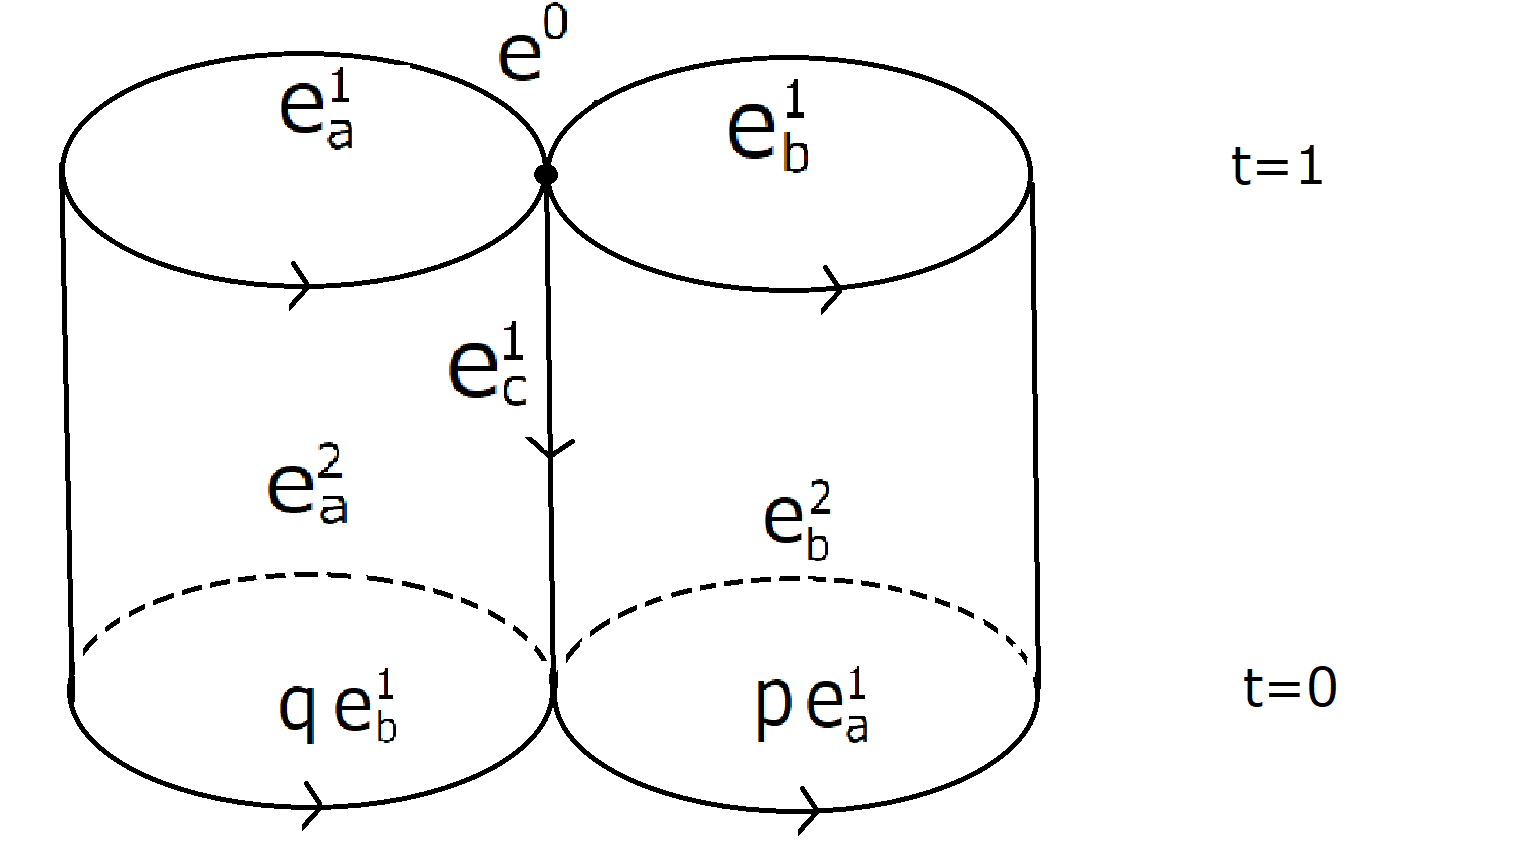
\includegraphics[width=5cm]{H31expert05_01.png}
\end{center}

この対になった円筒は、$X \tm I$および$Y$を表している。上下の円盤に見える部分は円周であり、ちくわを2つくっつけたような形をしている。側面も輪郭しか書かれていないが、面になっている。垂直方向が$I$成分を表しており、上が$t=1$で下が$t=0$であるものとしよう。また右を実軸のプラス方向、奥を虚軸のプラス方向とする。上部にある点は原点を表す。図に$e$と書かれているのはセルである。それぞれ具体的には次のように与えられる。
\begin{align*}
  e^0 &= (0,1) \\
  e^1_a &= \setmid{ (-1+e^{i\grt},1) }{0 < \grt < 2\pi } \\
  e^1_b &= \setmid{ (1-e^{i\grt},1) }{0 < \grt < 2\pi } \\
  e^1_c &= \setmid{ (0,t) }{0 < t < 1 } \\
  e^2_a &= \setmid{ (-1+e^{i\grt},t) }{0 < \grt < 2\pi , 0 < t < 1 } \\
  e^2_b &= \setmid{ (1-e^{i\grt},t) }{0 < \grt < 2\pi , 0 < t < 1 }
\end{align*}
このとき、次に注意する。
\begin{align*}
  e^0 &= (0,0) \\
  pe_a^1 &= \setmid{ (1-e^{i\grt},0) }{0 < \grt < 2\pi } \\
  qe_b^1 &= \setmid{ (-1+e^{i\grt},1) }{0 < \grt < 2\pi }
\end{align*}
さて以上の準備の下セル複体のホモロジーを計算しよう。$Y$の$0$セル、$1$セル、$2$セルの数はそれぞれ$1,3,2$個なので
\[
\xymatrix{
0 \ar[r] & \Z^2 \ar[r]^{\del} & \Z^3 \ar[r]^{\grs} & \Z \ar[r] & 0
}
\]
という図式に表されるような状況になっている。まず$\grs$だが、$0$セルはただひとつしかないのでこれはゼロ写像である。よって$H_0(Y)=\Z$がわかる。
次に$\del$を計算する。次の図

\begin{center}
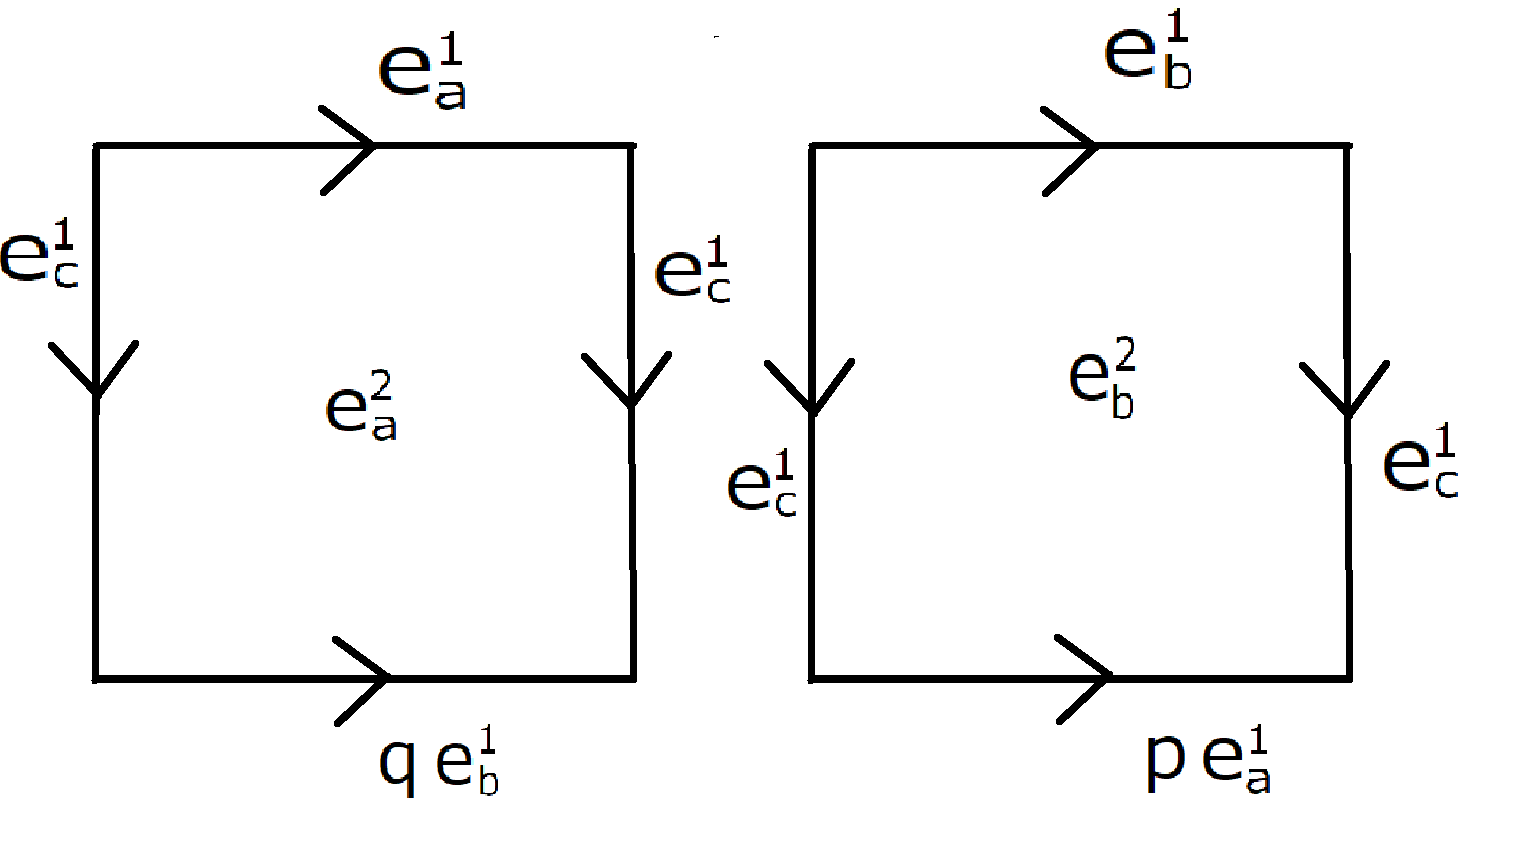
\includegraphics[width=5cm]{H31expert05_02.png}
\end{center}

のような状況になっているので
\[
\del(e_a^2) = e_a^1 - qe_b^1 \quad \del(e_b^2) = e_b^1 - pe_a^1
\]
である。したがって$\del$は次の行列
\[
\del = \pmat{
1 & -p \\
-q & 1 \\
0 & 0
}
\]
で表される写像である。この行列の階数は$pq =1$のとき$1$でそうでないとき$2$である。よって$pq = 1$のとき
\begin{align*}
  H_1(Y) &= \Z^3 / \Im \del \\
  &= \Z^2 \\
  H_2(Y) &= \Ker \del \\
  &= \Z
\end{align*}
である。$pq \neq 1$ならば
\begin{align*}
  H_1(Y) &= \Z^3 / \Im \del \\
  &= (a \Z \oplus  b \Z \oplus c \Z)  / (a - qb, b - pa) \\
  &= (a \Z \oplus  b \Z )  / ( (1-pq)a, b - pa) \oplus c \Z \\
  &= \Z / (1-pq)\Z \oplus \Z \\
  H_2(Y) &= \ker \del \\
  &= 0
\end{align*}
である。以上により求めるホモロジーは、$pq = 1$のとき
\[
H_i(Y) = \begin{cases}
\Z &(i=0,2) \\
\Z^2 &(i=1) \\
0 &(\text{otherwise})
\end{cases}
\]
であり、$pq \neq 1$のとき
\[
H_i(Y) = \begin{cases}
\Z &(i=0) \\
\Z / (pq-1)\Z \oplus \Z &(i=1) \\
0 &(\text{otherwise})
\end{cases}
\]
\end{sol}


\newpage


\section{平成30年度 基礎科目}

\subsubsection{} %{問1}
\lbar{
広義積分
\[
\iiint_V \f{1}{(1+x^2 + y^2)z^{ \f{3}{2} }} \; dx dy dz
\]
を計算せよ。ただし、$V=\setmid{(x,y,z) \in \R^3}{x^2+y^2 \leq z}$とする。
}

\begin{sol}
  極座標変換$(x,y,z) \mapsto (r,\grt, z)$を考える。このとき$dx dy dz = r dr d\grt dz$であり、
  \begin{align*}
    \iiint_V \f{1}{(1+x^2 + y^2)z^{ \f{3}{2} }} \; dx dy dz &= \int_{0}^{2\pi} \; d\grt \int_{0}^{\infty} \f{r}{1+r^2} \left( \int_{r^2}^{\infty} z^{ -\f{3}{2}  } \; dz \right) \; dr \\
    &= 2\pi \int_{0}^{\infty} \f{r}{1+r^2} \left[ (-2)z^{-\f{1}{2}} \right]^{\infty}_{r^2} \; dr \\
    &= 4\pi \int_{0}^{\infty} \f{r}{1+r^2} \f{1}{r} \; dr \\
    &= 4\pi \int_{0}^{\infty} \f{1}{1+r^2} \; dr \\
    &= 4\pi \cdot \f{\pi}{2} \\
    &= 2\pi^2
  \end{align*}
  と計算できる。
\end{sol}

\newpage

\subsubsection{} %{問2}
\lbar{
$a,b$を実数とする。実行列
\[
A = \begin{pmatrix}
1 & 1 & a & b \\
0 & 1 & 2 & 0 \\
2 & 0 & 1 & 4
\end{pmatrix}
\]
について、以下の問に答えよ。
\begin{description}
\item[(1)] 行列$A$の階数を求めよ。
\item[(2)] 連立1次方程式
\[
A \begin{pmatrix}
x_1 \\
x_2 \\
x_3 \\
x_4
\end{pmatrix} = \begin{pmatrix}
1 \\ 1 \\ 1
\end{pmatrix}
\]
が解を持つような実数$a,b$をすべて求めよ。
\end{description}
}

\begin{sol} ${}$
  \begin{description}
    \item[(1)] ある行に別の行の定数倍を足す操作を繰り返すと
    \begin{align*}
      A &\sim \begin{pmatrix}
      1 & 1 & a & b \\
      0 & 1 & 2 & 0 \\
      0 & -2 & 1-2a & 4-2b
      \end{pmatrix} \\
      &\sim \begin{pmatrix}
      1 & 1 & a & b \\
      0 & 1 & 2 & 0 \\
      0 & 0 & 5-2a & 4-2b
      \end{pmatrix}
    \end{align*}
    と変形できる。したがって$\rank A \geq 2$であり、$(a,b) = (\f{5}{2}, 2)$のときは$\rank A =2$で、$(a,b) \neq  (\f{5}{2}, 2)$のときは$\rank A =3$である。
    \item[(2)] $(a,b) \neq  (\f{5}{2}, 2)$ならば、$A \colon \R^4 \to \R^3$は全射なので、解がある。$(a,b) = (\f{5}{2}, 2)$のとき、拡大係数行列を考えると
    \begin{align*}
      \begin{pmatrix}
      1 & 1 & \f{5}{2} & 2 & 1 \\
      0 & 1 & 2 & 0  & 1 \\
      2 & 0 & 1 & 4 & 1
      \end{pmatrix} \sim
      \begin{pmatrix}
      1 & 1 & \f{5}{2} & 2 & 1 \\
      0 & 1 & 2 & 0  & 1 \\
      0 & -2 & -4 & 0 & -1
      \end{pmatrix}
      \sim \begin{pmatrix}
      1 & 1 & \f{5}{2} & 2 & 1 \\
      0 & 1 & 2 & 0  & 1 \\
      0 & 0 & 0 & 0 &  1
      \end{pmatrix}
    \end{align*}
    となるので、解はない。
  \end{description}
\end{sol}


\newpage

\subsubsection{} %{問 3}
\barquo{
広義積分
\[
\int_{-\infty}^{\infty} \f{\cos(\pi x)}{1 + x^2 + x^4} \; dx
\]
を求めよ。
}
\begin{sol}
$f$, $F$を
    \[
    f(x) = \f{\cos(\pi x)}{1 + x^2 + x^4}, \quad F(z) = \f{e^{\I \pi z}}{1 + z^2 + z^4}
    \]
により定める。$x \in \R$なら$f(x) = \Re F(x)$である。

ここで分母の$1 + z^2 + z^4$を因数分解しておく。
$\zeta = \exp(\I \pi / 3) = (1 + \sqrt{-3})/ 2$とする。$1+z + z^2$の根は$1$の原始$3$乗根であることから
\begin{align*}
  z^4 + z^2 + 1 &= (z^2 - \zeta^2)(z^2 - \zeta^4) \\
  &= (z - \zeta )(z + \zeta) (z - \zeta^2)(z + \zeta^2)
\end{align*}
である。

上反平面に含まれる半径$R$の半円を$C_R$とする。留数定理により、任意の$R > 1$について
\[
2 \pi \I ( \Res_{z=\zeta} F + \Res_{z=\zeta^2} F ) = \int_{-R}^R F(x) \; dx + \int_{C_R} f(z) \; dz
\]
が成り立つ。

ここで、
\begin{align*}
  \abs{\int_{C_R} f(z) \; dz } &\leq \int_0^{\pi} \abs{ \f{R \exp(\I R \pi e^{\I \grt}) }{ 1 + R^2e^{2 \I \grt} +  R^4e^{4 \I \grt}} } \; d\grt \\
  &\leq  \int_0^{\pi} \f{R e^{- R \pi \sin \grt} }{R^4 - R^2 - 1}   \; d\grt \\
  &\leq \f{R  }{R^4 - R^2 - 1}  \int_0^{\pi} \; d\grt \\
  &\leq  \f{R \pi }{R^4 - R^2 - 1}
\end{align*}
だから、$R \to \infty$のとき$\int_{C_R} f(z) \; dz \to 0$である。したがって
\[
 \int_{-\infty}^{\infty} f(x) \; dx =  \Re( 2 \pi \I ( \Res_{z=\zeta} F + \Res_{z=\zeta^2} F ) )
\]
であることがわかる。

実際に留数を計算しよう。詳細は省略するが、堅実な計算により
\begin{align*}
  \Res_{z=\zeta} F &= \f{ \exp(\I \pi \f{1 + \sqrt{-3}}{2} ) }{(2\zeta) (\zeta - \zeta^2) (\zeta + \zeta^2)  } \\
  &= \f{ - \I \exp(- \f{\sqrt{3}\pi}{2} ) }{2(1 - \zeta^2)} \\
  \Res_{z=\zeta^2} F &= \f{ \exp(\I \pi \f{-1 + \sqrt{-3}}{2} ) }{(\zeta^2 - \zeta) (\zeta^2 + \zeta) (\zeta^2 + \zeta^2)  } \\
  &=  \f{ - \I \exp(- \f{\sqrt{3}\pi}{2} ) }{2(1 + \zeta)}
\end{align*}
がわかる。$\gra = \exp(- \f{\sqrt{3}\pi}{2} )$とおこう。すると
\begin{align*}
  2 \pi \I ( \Res_{z=\zeta} F + \Res_{z=\zeta^2} F ) &= \gra \pi \left( \f{1}{1 - \zeta^2} + \f{1}{1+ \zeta} \right) \\
  &= \gra \pi \left( \f{2 - \zeta}{ 1 - \zeta^2} \right) \\
  &= \gra \pi
\end{align*}
である。$\gra \in \R$だから、
\[
 \int_{-\infty}^{\infty} f(x) \; dx = e^{- \f{\sqrt{3}\pi}{2} } \pi
\]
が結論される。
\end{sol}
\newpage

\subsubsection{} %{問 4}
\lbar{
閉区間$[0,1]$上の実数値関数列$\{ f_n \}^{\infty}_{n=1}$について、各$f_n$は広義単調増加であるものとする。つまり、$0 \leq x < y \leq 1$なら、$f_n(x) \leq f_n(y)$である。この関数列$\{ f_n \}^{\infty}_{n=1} $が$n \to \infty$で関数$f$に各点収束したとする。
\begin{description}
  \item[(1)] 任意の$0 \leq x < y \leq 1$に対し、不等式
  \[
  \sup_{x \in [x,y]} \abs{f_n(z) - f(z)} \leq \max\{ \abs{f_n(x)- f(y)}, \abs{f_n(y)-f(x)}  \}
  \]
  を示せ。
  \item[(2)] 関数$f$が連続であるとき、関数列$\{ f_n \}^{\infty}_{n=1}$は$f$に$[0,1]$上で一様収束することを示せ。
\end{description}
}
\begin{sol} ${}$
\begin{description}
  \item[(1)] まず$f$が広義単調増加であることを示す。$0 \leq x < y \leq 1$とする。$\ve > 0$が与えられたとする。$f_n$が$f$に各点収束することにより
  \begin{align*}
    n \geq N(x) \to \abs{f(x) - f_n(x)} < \ve \\
      n \geq N(y) \to \abs{f(y) - f_n(y)} < \ve
  \end{align*}
  なる$N(x), N(y)$の存在がわかる。したがって$n \geq \max\{ N(x), N(y) \}$のとき
  \begin{align*}
    f(y) - f(x) + 2\ve &= (f(y) + \ve ) - f(x) + \ve \\
    &\geq f_n(y) - f(x) + \ve &(-\ve < f(y)-f_n(y) < \ve \text{より}) \\
    &\geq f_n(y) - f_n(x) &(-\ve < f(x)-f_n(x) < \ve \text{より}) \\
    &\geq 0
  \end{align*}
  がわかる。$\ve > 0$は任意だったから、$f(y) \geq f(x)$がわかる。つまり$f$は広義単調増加である。

  したがって任意の$z \in [x,y]$に対して
\begin{align*}
f_n(z) - f(z) \leq f_n(y) - f(x) \\
f(z) - f_n(z) \leq f(y) - f_n(x)
\end{align*}
が成り立つので、
\[
\abs{f_n(z) - f(z)} \leq \max\{ \abs{f_n(x)- f(y)}, \abs{f_n(y)-f(x)}  \}
\]
である。右辺は$z$の取り方によらないので、
\[
\sup_{x \in [x,y]} \abs{f_n(z) - f(z)} \leq \max\{ \abs{f_n(x)- f(y)}, \abs{f_n(y)-f(x)}  \}
\]
がいえた。
\item[(2)] $\ve > 0$が与えられたとする。$I = [0,1]$はコンパクトなので、$f$は一様連続であることまでいえる。そこで
\[
\abs{x -y} < \grd \to \abs{f(x) - f(y)} < \ve
\]
なる$\grd > 0$がある。この$\grd$を固定し、$B(z) = [z - \grd/3, z + \grd/3] \cap I$とする。$\grd > 0$なので、$I = \bigcup_{i=1}^m B(z_i)$なる有限個の$z_i \in I$をとることができる。$B(z_i ) = [x_i, y_i]$と表すことにする。

$f_n$は$f$に各点収束しているので、
\begin{align*}
  n \geq N(x_i) &\to \abs{f(x_i) - f_n(x_i)} < \ve \\
  n \geq N(y_i) &\to \abs{f(y_i) - f_n(y_i)} < \ve
\end{align*}
なる$N(x_i), N(y_i)$がある。そこで
\[
n \geq \max\{ N(x_1), \cdots , N(x_m) , N(y_1) , \cdots , N(y_m)  \}
\]
とする。このとき
\begin{align*}
  \abs{f_n(x_i)- f(y_i) } &\leq \abs{ f_n(x_i) - f(x_i) } + \abs{ f(x_i) - f(y_i) } \\
  &\leq 2\ve \\
\abs{f_n(y_i)- f(x_i) }  &\leq \abs{ f_n(y_i) - f(y_i) } + \abs{ f(y_i) - f(x_i) } \\
&\leq 2\ve
\end{align*}
が成り立つ。したがって(1)により、不等式評価を端点に押しつけることができて
\begin{align*}
\sup_{z \in I } \abs{f_n(z) - f(z)} &\leq \max_{1 \leq i \leq m} \sup_{x \in [x_i,y_i]} \abs{f_n(z) - f(z)} \\
&\leq \max_{1 \leq i \leq m} \max\{ \abs{f_n(x_i)- f(y_i)}, \abs{f_n(y_i)-f(x_i)}  \} \\
&\leq 2\ve
\end{align*}
である。これで一様収束がいえた。
\end{description}
\end{sol}

\newpage

\subsubsection{} %{問 5}
\barquo{
$p$を素数とし、$\F_p = \Z / p \Z$を位数$p$の有限体とする。行列の乗法による群$G$を
\[
G = \setmid{ \pmat{1 & a & b \\ 0 & 1 & c \\ 0 & 0 & 1 } }{a,b,c \in \F_p}
\]
で定める。このとき、$G$から乗法群$\C^{\tm} = \C \sm \{ 0 \}$への準同形写像の個数を求めよ。
}
\begin{sol}
 次の事実に注意する。
\lem{
$\pi \colon G \to G/[G,G]$は自然な写像とする。すると$\pi$が誘導するAbel群の準同型
\[
p \colon \Hom(G/[G,G], \C^{\tm}) \to \Hom(G, \C^{\tm})
\]
は同型である。
}
\begin{proof}
$\pi$は全射なので、$p$は単射である。また$p$は全射でもある。なぜならば!$g \in \Hom(G, \C^{\tm})$が任意に与えられたとしよう。このとき$\C^{\tm}$がAbel群であることにより、$[G,G] \subset \Ker g$が成り立つ。したがって準同型定理により、$p(f) = g$となるような$f \in \Hom(G/[G,G], \C^{\tm})$が存在する。ゆえにかくのごとし。これで$p$が同型であることがいえた。
\end{proof}

 したがって$G/[G,G]$の構造を決定すればよい。そのためにまず$[G,G]$を決定する。
    \[
    A = \pmat{1 & a & b \\ 0 & 1 & c \\ 0 & 0 & 1},  \quad B = \pmat{1 & \grd & \beta \\ 0 & 1 & \grg \\ 0 & 0 & 1}
    \]
    とおく。($\gra$は$a$と間違えやすいので、$\grd$を使った。)計算すれば、このとき
    \begin{align*}
    ABA^{-1}B^{-1} = \pmat{1 & 0  & a \grg - c \grd \\ 0 & 1 & 0 \\ 0 & 0 & 1 }
  \end{align*}
  であることが判る。$a \grg - c \grd$は$\F_p$全体をわたるので、
  \[
  [G,G] = \setmid{ \pmat{1 & 0 & d \\ 0 & 1 & 0 \\ 0 & 0 & 1} }{d \in \F_p }
  \]
  が結論できる。

  次に$G/[G,G]$の構造を決定したい。
  \[
  E_1 = \pmat{1 & 1 & 0 \\ 0 & 1 & 0 \\ 0 & 0 & 1}, \quad E_2 =  \pmat{1 & 0 & 0 \\ 0 & 1 & 1 \\ 0 & 0 & 1}
  \]
  とし、$E_1, E_2 \in G/ [G,G]$と見なす。
  \[
  E_1^n = \pmat{1 & n & 0 \\ 0 & 1 & 0 \\ 0 & 0 & 1}, \quad E_2^m =  \pmat{1 & 0 & 0 \\ 0 & 1 & m \\ 0 & 0 & 1}
  \]
  なので、$E_1, E_2$は位数がちょうど$p$である。また、$C = E_1^n = E_2^m$とするとき
  \[
  1 = E_1^n E_2^{-m} = \pmat{ 1 & n & -nm \\ 0 & 1 & -m \\ 0 & 0 & 1}
  \]
  だから$n=m=0$が従う。つまり$\kakko{E_1} \cap \kakko{E_2} = 1$である。$G/[G,G]$はAbel群なので積による準同形
  $
\kakko{E_1} \tm \kakko{E_2} \to G/[G,G]
  $
  がある。これは、$\kakko{E_1} \cap \kakko{E_2} = 1$により単射である。位数$p^2$の有限群の間の単射なので、とくに同型である。よって$G/[G,G] \cong \F_p^2$がわかった。

あとは$\# \Hom(\F_p^2, \C^{\tm})$を求めよう。これは$\# \Hom(\F_p,\C^{\tm})$の$2$乗である。$\# \Hom(\F_p,\C^{\tm}) = p$より求める答えは$p^2$である。

\end{sol}

\newpage

\subsubsection{} %{問6}
\barquo{
$\R^4$の部分空間$M$を
\[
M = \setmid{(x,y,z,w) \in \R^4}{x^2 + y^2 + z^2 + w^2 = 1, \; xy + zw = 0}
\]
で定める。
\begin{description}
  \item[(1)] $M$が$2$次元微分可能多様体になることを示せ。
  \item[(2)] $M$上の関数$f$を
  \[
  f(x,y,z,w) = x
  \]
  で定めるとき、$f$の臨界点をすべて求めよ。ただし、$p \in M$が$f$の臨界点であるとは、$p$における$M$の局所座標$(u,v)$に関して
  \[
  \f{\del f}{\del u}(p) =   \f{\del f}{\del v}(p) = 0
  \]
  となることである。
\end{description}
}
\begin{sol} ${}$
  \begin{description}
    \item[(1)] $F \colon \R^4 \to \R^2$を
      \[
      F(x,y,z,w) = \pmat{x^2 + y^2 + z^2 + w^2 - 1 \\ xy+zw}
      \]
      により定める。$M = F^{-1}(O)$である。$p=(x,y,z,w) \in M$としよう。$p$におけるヤコビアンを計算すると
      \[
      JF_p = \pmat{2x & 2y & 2z & 2w \\ y & x & w & z }
      \]
      である。ここで$p \neq O$より$\rank JF_p \geq 1$である。仮に$\rank JF_p = 1$ならば、$JF_p$の2つの行は1次従属である。よって、$p \neq O$により$(y , x, w,z) = c(x,y,z,w)$なる定数$c \in \R$がある。このとき$xy + zw = c(x^2 + z^2) = 0$となり、$p \neq O$に矛盾。よって$\rank JF_p = 2$である。ゆえに$p$は$F$の正則点であり、$M$は$\R^4$の$2$次元部分多様体。
      $F$は$\bfC^{\infty}$級なので、$M$は微分可能になる。
      \item[(2)] $f \colon M \to \R$の$\R^4$への自然な拡張を$\wt{f}$とする。このとき$p \in M$に対して$T_p M \subset \R^4$と見なせば、$T_p M = \Ker JF_p$であるから、
      \begin{align*}
        \text{$p$が$f$の臨界点} &\iff \rank (df_p \colon T_p M \to \R) < 1 \\
        &\iff \dim \Ker df_p = 2 \\
        &\iff \dim \Ker \pmat{JF_p \\ J\wt{f}_p} = 2 \\
        &\iff \rank \pmat{2x & 2y & 2z & 2w \\ y & x & w & z \\ 1  & 0 & 0 & 0} = 2 \\
        &\iff \rank \pmat{0 & 2y & 2z & 2w \\ 0 & x & w & z \\ 1  & 0 & 0 & 0} = 2
      \end{align*}
      である。いま$p=(x,y,z,w) \in M$が臨界点であったと仮定する。このとき$(x,w,z)$と$(y,z,w)$は1次従属である。よって$(y,w,z) = 0$かまたは、ある$c \in \R$が存在して$(x,w,z)=  c(y,z,w )  $である。$(y,w,z) = 0$なら$p =(\pm 1, 0, 0 ,0)$である。$(x,w,z)=  c(y,z,w )  $なら、$c(y^2 + z^2)=0$より$p=(0, \pm 1, 0, 0)$である。

      逆に$p=(\pm 1, 0, 0 ,0), (0, \pm 1, 0, 0)$ならば$p \in M$であり、$f$の臨界点であることはあきらかなので、臨界点はこれですべて求まったことになる。
  \end{description}

\end{sol}


\newpage

\subsubsection{} %{問7}
\barquo{
$A$を実正方行列、$k$を正の整数とし、$\rk (A^{k+1}) = \rk (A^k)$が成り立つとする。このとき、任意の整数$m \geq k$に対し、$\rk (A^m) = \rk (A^k)$であることを証明せよ。ここで行列$X$に対し、$\rk(X)$は$X$の階数を表す。
}
\begin{proof}
  仮定から、$\Ker A^{k+1}$の次元と$\Ker A^k$の次元は等しい。包含関係があって次元が等しいので、$\Ker A^{k+1} = \Ker A^k$である。ここで$m \geq k +2$に対して$x \in \Ker A^m$と仮定する。そうすると$A^m x = A^{m-k-1} A^{k+1} x$だから$A^{m-k-1} x \in \Ker A^{k+1} = \Ker A^k$である。よって$A^k A^{m-k-1} x = A^{m-1} x = 0$であり、$x \in \Ker A^{m-1}$がわかる。これを帰納的に繰り返して、
  $\Ker A^m \subset \Ker A^{m-1} \subset \cdots \subset \Ker A^k$を得る。逆はあきらかなので$\Ker A^m = \Ker A^k$である。よってとくに階数も等しい。
\end{proof}


\newpage

\bfsection{平成30年度 専門科目}

\bfsubsection{問1}
\barquo{
$k$を可換体とする。$k[X,Y]$を$k$上の2変数多項式環として、$f \in k[X,Y]$の零点集合$V(f)$を
\[
V(f) = \setmid{(a,b) \in k \tm k}{f(a,b) = 0}
\]
によって定義する。次の2条件は同値であることを示せ。
\begin{description}
  \item[(1)] $k$は代数的閉体ではない。
  \item[(2)] $V(f) = \{(0,0)\}$となる$f \in k[X,Y]$が存在する。
\end{description}
}
\begin{sol}${}$
\begin{description}
  \item[(1)$\To$(2)] $k$は代数的閉体ではないので、ある1次以上の多項式$g \in k[X]$であって、$k$上根を持たないものが存在する。$n = \rm{dim}\ g$とおいて、
  \[
  f(X,Y)= Y^n g \left(\frac{X}{Y} \right)
  \]
  とおく。別の言い方をすれば$g(X)= X^n + a_{n-1}X^{n-1} + \cdots + a_1X + a_0$とするとき, $f(X,Y)= X^n + a_{n-1}X^{n-1}Y + \cdots + a_1XY^{n-1} + a_0Y^n$である。$X \in k$, $Y \in k \sm \{0\}$に対して$Y^n$と$g(X/Y)$は決して0にならないので、$f(X,Y)=0$となるのは$Y=0$のときだけである。$f(X,0)=X^n$なので、
  $V(f) =\{ (0,0)\}$が成り立つ。
  \item[(2)$\To$(1)] 対偶をとり、$k$が代数閉体であってかつ$V(f) =\{ (0,0)\}$となる$f \in k[X,Y]$が存在すると仮定し矛盾を示そう。このとき$k$は無限体($k$が有限体であっても、アイゼンシュタイン多項式は無限個あるため)であることに注意する。またここではそもそも$k$は零環ではないとして考えていることにも注意する。

  さて$a,b \in k^{\tm}$を任意にとると、$f(a,Y) \in k[Y]$、$f(X,b) \in k[X]$は決して0にならないので、定数でなければならない。
  このとき$f(a,Y)=f(a,b)=f(X,b)$であるので、常にこの2つは一致する。割り算を実行して
  \begin{align*}
    f(X,Y) &= (X-a)g(X,Y) + f(a,Y) \\
    f(X,Y) & =(Y-b)h(X,Y)+f(X,b)
  \end{align*}
  なる$g, h \in k[X,Y]$をとってくる。すると辺々引いて
  \[
  0 = (X-a)g(X,Y) - (Y-b)h(X,Y)
  \]
  が成り立つ。この等式は任意の$a,b \in k^{\times}$について成り立つので、$g=h=0 \in k[X,Y]$が判る。ゆえに$f$は定数となるがこれは矛盾。
  \item[別解] (2)$\To$(1)を示す部分についてはHilbertの零点定理を知っていればすこし議論を省略できる。$k$が代数閉体だと仮定し$V(f) =\{ (0,0)\}$となる$f \in k[X,Y]$が存在するとしよう。$k[X,Y]$はUFDなので、$f$は既約であるとしてよい。すると$(f)$は根基イデアルなのでHilbertの零点定理により$(f) = (X,Y)$である。しかし右辺は単項イデアルではないので矛盾。
\end{description}
\end{sol}


\newpage





\bfsubsection{問2}
\barquo{
$p$を素数, $k,m$を正の整数で、$k$と$p^2 - p$は互いに素であるとする。位数$kp^m$の有限群$G$が次の性質を満たす部分群$N,H$をもつとする。
\begin{description}
  \item[(1)] $N$は位数$p^m$の巡回群で$G$の正規部分群である。
  \item[(2)] $H$は位数$k$の群である。
\end{description}
このとき、$G$は$N$と$H$の直積であることを示せ。
}
\begin{sol}
  $H \lhd G$を示せば十分である。(付録の「半直積とGaois群」を参照のこと) $N \lhd G$なので、$H$の共役による$N$への作用$\Phi \colon H \rightarrow \Aut N$を$\Phi_h(q)=hqh^{-1}$により定義できる。$H / \Ker \Phi$は$\Aut N$の部分群とみなせる。
  \begin{align*}
    \#(\Aut N) &= \#((\Z/ p^m \Z)^{\tm}) \\
    &= p^m - p^{m-1}
  \end{align*}
  なので、$\#(H / \Ker \Phi)$は$\# H= k$と$ p^m - p^{m-1}$の両方を割り切る。したがって$\#(H / \Ker \Phi) \leq \gcd (k,p^m - p^{m-1})$であるが、右辺は仮定により1だから$\Phi$は自明な作用であって、$H$の元はすべての$N$の元と可換である。

  よって、$G$の元$g=hq \; (h \in H, q \in N)$と$x \in H$に対して$g^{-1}xg = x^g =x^{hq} = (x^h)^q = x^h \; \in H$だから、$H \lhd G$が言えた。
\end{sol}

\newpage


\bfsubsection{問3}
\barquo{
多項式$X^7 - 11$の有利数体$\Q$上の最小分解体を$K \subset \C$とする。このとき、次の問に答えよ。
\begin{description}
  \item[(1)] 拡大次数$[K:\Q]$を求めよ。
  \item[(2)] $\Q$と$K$の間の($\Q$でも$K$でもない)真の中間体の個数を求めよ。
  \item[(3)] 上記(2)の中間体のうち、$\Q$上Galois拡大になるものの個数を求めよ。
\end{description}
}
\begin{sol} ${}$
\begin{description}
  \item[(1)] $\gro = \exp (2\pi \sqrt{-1}/7)$とする。あきらかに$K = \Q(\gro, \sqrt[7]{11})$である。状況を図式で表すと次のようになる。
  \[
  \xymatrix{& K &  \\  \Q(\gro) \ar[ur]^{\leq 7} & & \Q(\sqrt[7]{11}) \ar[ul]_{\leq 6} \\  &  \Q \ar[ul]^{6} \ar[ur]_{7} &
  }
  \]
  円分体の一般論から$6= [\Q(\gro):\Q]$である。また$X^7 - 11$はEisenstein多項式なので既約であり$7=[\Q(\sqrt[7]{11}):\Q]$である。$7$と$6$は互いに素なので$\Q(\gro) \cap \Q(\sqrt[7]{11}) = \Q$である。
  $\Q(\gro) / \Q$はGalois拡大なので、Galois拡大の推進定理により$\Gal(K/ \Q(\sqrt[7]{11})) \cong \Gal(\Q(\gro) / \Q)$であり、とくに$[K: \Q(\sqrt[7]{11})] = [\Q(\gro):\Q] = 6$である。したがって、$[K:\Q]=42$である。
  \item[(2)] $G = \Gal(K/ \Q)$とする。付録「半直積とGalois群」により、$G$は半直積
  \[
\Gal(K/ \Q(\gro)) \rtimes \Gal(K/ \Q(\sqrt[7]{11}))
  \]
  と同型である。素数次数なので$\Gal(K/ \Q(\gro)) = \Z / 7 \Z$であり、
  円分体の一般論から
\[
\Gal(K/ \Q(\sqrt[7]{11})) \cong \Gal(\Q(\gro) / \Q) = (\Z / 7 \Z)^{\tm} = \Z / 6 \Z
\]
  である。つまりともに有限巡回群である。$\grs \in \Gal(K/ \Q(\gro))$を$\grs(\sqrt[7]{11}) = \sqrt[7]{11} \gro$により定め、
  $\tau \in \Gal(K/ \Q(\sqrt[7]{11}))$を$\tau(\gro) = \gro^3$により定める。$\grs$, $\tau$はそれぞれ生成元となる。$\tau \grs \tau^{-1}(\sqrt[7]{11}) = \sqrt[7]{11} \gro^3$より
  $\tau \grs \tau^{-1} = \grs^3$である。したがって次の表示
  \[
  G \cong \setmid{\grs,\tau}{\grs^7 = \tau^6 = 1, \tau \grs \tau^{-1} = \grs^3} \cong \Z / 7 \Z \rtimes \Z / 6 \Z
  \]
  を得る。

  Galoisの基本定理により、$G$の自明でない部分群の個数を求めればよい。そこでまずすべての元の位数を決定する。$\kakko{\grs} \rtimes \kakko{\tau} \to \kakko{\tau}$は群準同型なので、$x = \grs^i \tau^j \in G$の共役は$\grs^{*} \tau^j$という形をしている。具体的には
    \begin{align*}
      \grs x \grs^{-1} &= \grs \grs^i \tau^j \grs^{-1} \\
      &= \grs \grs^i (\tau^j \grs^{-1} \tau^{-j} ) \tau^j \\
      &= \grs \grs^i (\grs^{3^j})^{-1} \tau^j \\
      &= \grs^{1 - 3^j} \grs^i \tau^j \\
      &= \grs^{1 - 3^j} x
    \end{align*}
    である。
  そこで共役元を求めることにより次のような位数の表をつくることができる。
  \begin{center}
  \begin{tabular}{ccc}
   \hline
位数 & 元 & 個数 \\
   \hline \hline
   1 & 1 & 1 \\
   2 & $\grs^i \tau^3 \; (0 \leq i \leq 6)$ &  7 \\
  3 & $\grs^i \tau^2 \; (0 \leq i \leq 6)$, $\grs^i \tau^4 \; (0 \leq i \leq 6)$ &  14  \\
  6 & $\grs^i \tau \; (0 \leq i \leq 6)$, $\grs^i \tau^5 \; (0 \leq i \leq 6)$ & 14 \\
  7 & $\grs^i \; ( 1 \leq i \leq 6)$ & 6
   \end{tabular}
  \end{center}
  次に部分群を列挙する作業に移る。$G$の位数は42なので、自明でない部分群の位数としてありえるのは$2,3,6,7,14,21$である。まず位数2の部分群は位数2の元と同じ数だけあるので、7個である。位数3の部分群は、素数位数なのですべて巡回群であり、生成元はひとつの群に対して2つある。よって位数3の部分群は$14/2 = 7$個ある。

  位数6の部分群$M \subset G$が与えられたとする。このとき次のような各行が完全な可換図式がある。
\[
\xymatrix{
1 \ar[r] & \Z / 7 \Z \ar[r]^-j &  \Z / 7 \Z \rtimes \Z / 6 \Z \ar[r]^-p & \Z / 6 \Z \ar[r] & 1 \\
1 \ar[r] & j^{-1}(M) \ar[r]^-j  \ar[u] & M  \ar[u] \ar[r]^-p & p(M) \ar[r] \ar[u] & 1
}
\]
$j^{-1}(M) = 1$でなくてはならないため、$M \cong p(M)$でありしたがって$M$は巡回群である。位数6の巡回群の生成元はひとつの群に対して2つなので、位数6の部分群は$14/2 = 7$個ある。
  位数7の部分群は、Sylow-7部分群なのですべて共役である。ところが$\kakko{\grs}$は正規部分群だったので、ひとつしかない。
  位数14の部分群は、Sylowの定理より位数2の元と位数7の元で生成される。したがって$\kakko{\grs, \tau^3}$しかない。よって1個。位数21の部分群も、Sylowの定理により位数3の元と位数7の元で生成される。したがって$\kakko{\grs, \tau^2}$しかない。よって1個。以上により、次の表のようになる。
  \begin{center}
  \begin{tabular}{ccc}
   \hline
位数 & 部分群 & 個数 \\
   \hline \hline
   2 & $\kakko{\grs^i \tau^3}  \; (0 \leq i \leq 6)$ &  7 \\
  3 & $\kakko{\grs^i \tau^2} \; (0 \leq i \leq 6)$ &  7  \\
  6 & $\kakko{\grs^i \tau} \; (0 \leq i \leq 6)$ & 7 \\
  7 & $\kakko{\grs}$ & 1 \\
  14 & $\kakko{\grs, \tau^3}$ & 1 \\
  21 & $\kakko{\grs, \tau^2}$ & 1
   \end{tabular}
  \end{center}
  したがって非自明な部分群は$7 + 7 + 7 + 1 + 1 + 1 = 24$個ある。
  \item[(3)] Galoisの基本定理により、$G$の自明でない正規部分群の個数を求めればよい。$x = \grs^i \tau^j \in G$の共役$\grs x \grs^{-1}$は$\grs^{1 - 3^j} x$
    であることを思い出そう。これをみると、位数$2,3,6$の群のなかに正規部分群は存在しない。また、位数7,14,21の群はすべて正規部分群である。よって自明でない正規部分群は3個である。
\end{description}
\end{sol}


\newpage

\section{平成29年度 基礎科目}

\subsubsection{} %{問1}
\barquo{
次の重積分を求めよ。
\[
\iint_D e^{- \max \{ x^2,y^2 \} } \ dx dy
\]
ここで$D=\setmid{(x,y) \in \R^2}{0 \leq x \leq 1, 0 \leq y \leq 1}$とする。
}
\begin{sol}
  $E = \setmid{(x,y) \in D}{x \geq y}$とおく。このとき
  \begin{align*}
    \iint_D e^{- \max \{ x^2,y^2 \} } \ dx dy &= 2 \iint_E e^{- x^2 } \ dx dy \\
    &= 2 \int_0^1 \left(  \int_0^x e^{-x^2} \ dy   \right) \ dx \\
    &= 2 \int_0^1 x e^{-x^2} \ dx \\
    &= \int_0^1 e^{-z} \ dz &(z = x^2 \text{とおいた}) \\
    &= 1 - e^{-1}
  \end{align*}
\end{sol}


\newpage


\subsubsection{} %{問2}
\barquo{
実行列
\[
A= \pmat{
1 & -2 & -1 & 1 & 0 \\
-2 & 5 & 3 & -2 & 1 \\
1& 1& 2 &0 &-1 \\
5&  0&  5&  3&  2 \\
}
\]
について、以下の問に答えよ。
\begin{description}
  \item[(i)] 連立一次方程式
  \[
  A \pmat{
  x_1 \\
  x_2 \\
  x_3 \\
  x_4 \\
  x_5
  }
  = \pmat{ 0\\ 0\\ 0\\ 0 }
  \]
  の解をすべて求めよ。
  \item[(ii)]
  連立一次方程式
  \[
  A \pmat{
  x_1 \\
  x_2 \\
  x_3 \\
  x_4 \\
  x_5
  }
  = \pmat{0 \\ -1 \\ 1\\  c}
  \]
  が解を持つような実数$c$をすべて求めよ。
\end{description}
}
\begin{sol} ${}$
  \begin{description}
    \item[(i)] 行列$A$に行基本変形を繰り返し行っていく。
    \begin{align*}
      A &= \pmat{
      1 & -2 & -1 & 1 & 0 \\
      -2 & 5 & 3 & -2 & 1 \\
      1& 1& 2 &0 &-1 \\
      5&  0&  5&  3&  2 \\
      } \\
      &\sim \pmat{
      1 & -2 & -1 & 1 & 0 \\
      0 & 1 & 1 & 0 & 1 \\
      0& 3& 3 &-1 &-1 \\
      0&  10&  10&  -2&  2 \\
      } & \pmat{ R_1 \\ R_2+2R_1 \\ R_3-R_1 \\ R_4-5R_1} \\
     &\sim \pmat{
      1 & 0 & 1 & 1 & 2 \\
      0 & 1 & 1 & 0 & 1 \\
      0& 0& 0 &-1 &-4 \\
      0&  0&  0&  -2&  -8 \\
      } & \pmat{ R_1+2R_2 \\ R_2 \\ R_3-3R_2  \\ R_4 -10R_2} \\
      &\sim \pmat{
        1 & 0 & 1 & 0 & -2 \\
        0 & 1 & 1 & 0 & 1 \\
        0& 0& 0 &1 &4 \\
        0&  0&  0&  0&  0 \\
        } & \pmat{R_1+R_3 \\ R_2 \\ -R_3 \\ R_4-2R_3 }
    \end{align*}
    したがって、$A\bfx=\bfzero$の解空間は$x_3,x_5 \in \R$で貼られる$2$次元実ベクトル空間
    \[
    S = x_3 \pmat{-1 \\-1 \\1 \\0 \\0 } + x_5 \pmat{2\\ -1\\ 0\\ -4\\ 1}
    \]
    である。
    \item[(ii)] 次の事実に気を付ける。
    \prop{
    $k$は体、$A$は$k$係数の$(n,m)$行列であり$\bfx \in k^m, \bfb \in k^n$であるとする。このとき$\bfx$についての一次方程式$A\bfx = \bfb$が解を持つことと、$\rank A = \rank (A \; \bfb)$は同値。
    }
    \begin{proof}
      まず次は同値である。
      \[
        \exists \bfx \; A\bfx = \bfb \iff \exists \bfx \;  \pmat{A & \bfb} \pmat{\bfx \\ -1} = \bfzero
      \]
      ここで、$\Ker A \to \Ker (A \; \bfb) \st \bfx \mapsto {}^t(\bfx \; 0)$によって$\Ker A$は$\Ker (A \; \bfb)$の部分空間$\Ker (A \; \bfb) \cap \setmid{\bfy \in k^{m+1}}{y_{m+1}=0}$だと思えることに気を付けると
      \begin{align*}
      \exists \bfx \; A\bfx = \bfb &\iff \dim \Ker (A \; \bfb) > \dim  \Ker A \\
        &\iff 0 \leq \rank (A \; \bfb) - \rank A < 1 \\
        &\iff \rank A = \rank (A \; \bfb)
      \end{align*}
      であることがわかる。
    \end{proof}
    (ii)の解答に戻る。$\bfb = {}^t(0 \ -1 \;  1 \; c)$とおく。拡大係数行列$(A \; \bfb)$は行基本変形により
    \[
    (A \; \bfb) \sim \pmat{1& 0& 1&  0& -2& 2 \\ 0 &1& 1& 0& 1& -1 \\ 0& 0& 0& 1& 4& -4 \\ 0& 0& 0& 0& 0& c+2}
    \]
    と変形できる。したがって求める$c$の値は$c=-2$である。
  \end{description}
\end{sol}





\newpage





\subsubsection{} %{問3}
\barquo{
$m,n$を正の整数とし、$A$を複素$(n,m)$行列、$B$を複素$(m,n)$行列とする。複素数$\grl \neq 0$について、以下の問に答えよ。
\begin{description}

  \item[(i)] $\grl$が$BA$の固有値ならば、$\grl$は$AB$の固有値でもあることを示せ。
  \item[(ii)] $\C^m$, $\C^n$の部分空間$V,W$をそれぞれ
\begin{align*}
  V &= \setmid{\bfx \in \C^m}{ \text{ある正の整数$k$に対して} (BA - \grl I_m)^k \bfx = \bfzero \text{が成り立つ} } \\
  W &= \setmid{\bfy \in \C^n}{ \text{ある正の整数$l$に対して} (AB - \grl I_n)^l \bfy = \bfzero \text{が成り立つ} }
\end{align*}
で定める。ただし、$I_m,I_n$は単位行列、$\bfzero$は零ベクトルを表す。このとき、$\dim V = \dim W$であることを示せ。
\end{description}
}
\begin{sol} ${}$
  \begin{description}
    \item[(i)] $BA \bfv = \grl \bfv$なる$\bfv \neq \bfzero$があったとする。このとき
    \begin{align*}
      AB(A \bfv) &= A(BA \bfv) \\
      &= A (\grl \bfv) \\
      &= \grl A \bfv
    \end{align*}
    である。もしも$A \bfv = \bfzero$ならば$\grl \bfv = \bfzero$となり矛盾。したがって$A \bfv \in \C^n$は$AB$の固有ベクトルである。
    \item[(ii)] $M = AB, N = BA$とする。$MA = AN$である。いま$\bfx \in V$とする。ある$k$が存在して$(N - \grl I_m)^k \bfx = \bfzero$である。このとき
    \[
(M - \grl I_n)^k (A \bfx) = A  (N - \grl I_m)^k \bfx = \bfzero
    \]
    であるから$A \bfx \in W$である。したがって行列$A$は線形写像$A \colon V \to W$であるとみなせる。このとき$A$は$V$の定義および$\grl \neq 0$により単射だから、$\dim V \leq \dim W$である。同様にして逆が言えるので$\dim V = \dim W$が従う。
  \end{description}
\end{sol}

\newpage


\subsubsection{} %{問4}
\barquo{
$f$を$I=\setmid{x \in \R}{x \geq 0}$上の実数値連続関数とする。正の整数$n$に対し、$I$上の関数$f_n$を
\[
f_n(x)=f(x+n)
\]
で定める。関数列$\{  f_n \}_{n=1}^{\infty}$が$I$上で一様収束するとき、以下の問に答えよ。
\begin{description}
\item[(i)] $I$上の関数$g$を
\[
g(x) = \lim_{n \to \infty} f_n(x)
\]
で定める。このとき$g$は$I$上で一様連続であることを示せ。
\item[(ii)] $f$は$I$上で一様連続であることを示せ。
\end{description}
}
\begin{sol} 以下$I$上の連続関数$h$に対してその一様ノルムを$\norm{h} = \sup_{x \in I} \abs{h(x)}$とかく。
  \begin{description}
    \item[(i)] 連続関数$f_n$の一様極限なので$g$は連続である。さらに定義より$g(x+1)=g(x)$だから、$g$はコンパクト集合$\R / \Z$上の連続関数であるとみなせ、したがって一様連続である。
    \item[(ii)] $\ve > 0$が与えられたとする。$g$の一様連続性から
    \[
    \forall x,y \in I \; \abs{x-y}< \grd_0 \to \abs{g(x) - g(y) } < \ve
    \]
    なる$\grd_0 > 0$がある。$f_n$は$g$に一様収束するので
    \[
    n \geq N \to \norm{f_n - g} < \ve
    \]
    なる$N \in \Z$がある。このとき
    \[
    \forall x,y \in [N,\infty) \; \abs{x - y } < \grd_0 \to \abs{f(x) - f(y)} \leq 3\ve
    \]
    が成り立つ。なぜなら
    \[
    \abs{f(x) - f(y)}  \leq \abs{f_N(x-N) - g(x-N)} + \abs{g(x)-g(y)} + \abs{g(y-N)-f_N(y-N)}
    \]
    であるから。また$f$は連続なので、コンパクト集合$[0,N]$上ではとくに一様連続である。したがって
    \[
    \forall x,y \in [0,N] \; \abs{x - y } < \grd_1 \to \abs{f(x) - f(y)} \leq \ve
    \]
    なる$\grd_1 > 0$がある。したがって$\grd= \min_i{\grd_i}$とすると
    \[
    \forall x,y \in I \; \abs{x - y } < \grd \to \abs{f(x) - f(y)} \leq 4\ve
    \]
    であり、これで$f$が$I$上一様連続であることがいえた。
  \end{description}
\end{sol}






\newpage



\subsubsection{} %{問5}
\barquo{
$p$を正の実数とし、$f(t)$を$\R$上の実数値連続関数で
\[
\int_0^{\infty} \abs{f(t)} \ dt < \infty
\]
を満たすものとする。このとき$\R$上の常微分方程式
\[
\f{dx}{dt} = -px + f(t)
\]
の任意の解$x(t)$に対し$\lim_{t \to \infty} x(t) = 0$が成り立つことを示せ。
}
\begin{sol}
  任意に$\ve > 0$が与えられたとする。仮定により
  \[
  \int_R^{\infty}  \abs{f(t)} \ dt < \ve
  \]
  となるような$R \geq 0$がある。$x = y e^{-pt}$と置いて変数変換をすると
  \[
  \f{dy}{dt} = e^{pt}f(t)
  \]
  となる。よってある定数$C$により
  \[
  y(t) = \int_0^t f(s)e^{ps} \ ds + C
  \]
と表せる。$C$の値は$t \to \infty$での$x$の振る舞いに関与しないので、はじめから$C=0$と仮定してよい。これにより
\[
x(t) =   \int_0^t f(s)e^{p(s-t)} \ ds
\]
であることがわかる。そこで$M =  \int_0^R \abs{f(s)} \ ds $とおき、$ t > \max \{ R, R+ \f{1}{p} \log \f{M}{\ve} \}$とする。このとき
\begin{align*}
  \abs{x(t)} &\leq \int_0^R \abs{f(s)}e^{p(s-t)} \ ds  + \int_R^t \abs{f(s)}e^{p(s-t)} \ ds  \\
  &\leq e^{p(R-t)} M + \int_R^t \abs{f(s)} \ ds  \\
  &\leq \ve  + \int_R^{\infty} \abs{f(s)}  ds \\
  &\leq 2\ve
\end{align*}
である。よって$\lim_{t \to \infty} x(t) = 0$である。
\end{sol}



\newpage





\subsubsection{} %{問6}
\barquo{
$X,Y$を位相空間とし、直積集合$X \tm Y$を積位相によって位相空間とみなす。写像$f \colon X \tm Y \to Y$を$f(x,y)=y$で定める。$X$がコンパクトならば、$X \tm Y$の任意の閉集合$Z$に対し、$f(Z)$は$Y$の閉集合であることを示せ。
}
\begin{rem}
  $X$がコンパクトという仮定は必要である。例えば、$X=Y=\R$かつ$Z=\setmid{(x,y) \in \R^2}{xy=1}$としてみればわかる。
\end{rem}
\begin{sol}
$Y \sm f(Z)$の元$y$が任意に与えられたとする。このとき$f^{-1}(y) \subset X \tm Y \sm Z$である。ここで$Z$が$X\tm Y$の閉集合という仮定から、$X \tm Y \sm Z \opsub X \tm Y$である。したがって積位相の定義により、ある開集合の族$U_i \subset X$と$V_i \subset Y$であって$X \tm Y \sm Z = \bigcup_{i \in I} U_i \tm V_i$なるものがある。
$f^{-1}(y) = X \tm \{ y \} \cong X$はコンパクトであると仮定したので、ある有限集合$J \subset I$が存在して$X \tm \{y\} = f^{-1}(y) \subset \bigcup_{i \in I} U_i \tm V_i$が成り立つ。

ここで$V = \bigcap_{i \in J} V_i$とおく。$J$は有限集合なので$V$は$Y$の開集合であり、かつ$y$を含む。また$X = \bigcup_{i \in J} U_i$であることより$Z \cap f^{-1}(V) = Z \cap (X \tm V) = Z \cap \bigcup_{i \in J} (U_i \tm V) \subset Z \cap (X \tm Y \sm Z) = \emptyset$となる。
これは$V \cap f(Z) = \emptyset$を意味し、$y$は内点であったことがわかった。よって$f(Z)$は$Y$の閉集合。
\end{sol}


\newpage

\subsubsection{} %{問7}
\barquo{
$n$を正の整数とし、$\R^n$の2点$x=(x_1, \cdots , x_n)$, $y= (y_1, \cdots , y_n)$の距離$d(x,y)$を
\[
d(x,y) = \sqrt{(x_1 - y_1)^2 + \cdots +  (x_n - y_n)^2}
\]
と定める。$\R^n$の空でない部分集合$A$に対し、関数$f \colon \R^n \to \R$を
\[
f(x) = \inf_{z \in A} d(x,z)
\]
で定めるとき、$\R^n$の任意の2点$x,y$に対して$\abs{f(x)-f(y)} \leq d(x,y)$が成り立つことを示せ。
}
\begin{sol}
  $d(x,0) = \abs{x}$と書くことにする。任意に$\ve > 0$が与えられたとしよう。このとき$f$の定義から、$f(y) + \ve > \abs{y-w} \geq f(y)$なる$w \in A$が存在する。このとき$f(x) \leq \abs{x-w}$が成り立つので、
  \begin{align*}
    f(x) - f(y) - \ve &\leq f(x) - \abs{y-w} \\
    &\leq \abs{x-w} - \abs{y-w} \\
    &\leq \abs{x-y}
  \end{align*}
  である。$\ve > 0$は任意だったので、$f(x) - f(y) \leq \abs{x-y}$でなくてはならない。同様にして$f(x) - f(y) \leq \abs{x-y}$がいえるので、示すべきことがいえた。
\end{sol}


\newpage


\bfsection{平成29年度 専門科目}

\bfsubsection{問1}
\barquo{
$G$を有限群とする。$G$の自己準同形全体のなす群を$\Aut (G)$とおく。また、$G$および$\Aut (G)$の位数をそれぞれ$a= |G|$, $b= |\Aut G|$とおく。以下の問に答えよ。
\begin{description}
  \item[(i)] $b=1$のとき、$G$は自明群であるか、または$\Z / 2 \Z$と同型であることを示せ。
  \item[(ii)] $a$が奇数で$b=2$となるような$G$をすべて求めよ。
\end{description}
}
\begin{sol} この解答では集合の元の個数を$\#$で表記する。
   \begin{description}
     \item[(i)] 群準同形$\phi \colon G \to \Aut G$を$\phi_g(x)=gxg^{-1}$により定める。$\# \Aut G = 1$という仮定より、$G = \Ker \phi = Z(G)$である。したがって$G$はAbel群。よって有限生成Abel群の基本定理により、ある素数の集合$M \subset \Z$と写像$I \colon M \to P(\Z)$が存在して
     \[
     G = \bigoplus_{p \in M} \bigoplus_{i \in I(p)} \Z / p^{e_i} \Z
     \]
     と表すことができる。このとき乗法群$(\prod_{p, i } \Z / p^{e_i} \Z)^{\tm}$は$\Aut G$の部分群とみなせるので
     \[
     \prod_{p, i} p^{e_i - 1}(p -1) = 1
     \]
     である。したがって$M=\{ 2 \}$である。また任意の$i \in I(2)$に対して$e_i = 1$である。よって$G = (\Z / 2 \Z)^n$と表せるが、$\Aut G = 1$という仮定から$n=1$でなくてはならない。($n \geq 2$なら、たとえば順番を入れ替える写像などがある)
     \item[(ii)] 仮定から$G/ Z(G) = G/ \Ker \phi $の位数は2以下である。写像$f \colon G \to G$を$f(x) = x^2$で定義する。$x,y \in G$に対して、もしも$x \in Z(G)$または$y \in Z(G)$ならば$f(xy)=f(x)f(y)$である。また$x , y \in G \sm Z(G)$であれば、$xy \in Z(G)$なので$f(xy)=xy(xy) =f(x)f(y)$である。したがって$f$は群準同形となる。$\# G$は奇数なので$f$は単射であり、位数の考察から同型となる。このことから結局$G= Z(G)$であり、$G$はAbel群である。ゆえに有限生成Abel群の基本定理から
     \[
        G = \bigoplus_{p \in M} \bigoplus_{i \in I(p)} \Z / p^{e_i} \Z
     \]
     と表すことができる。このとき乗法群$(\prod_{p, i } \Z / p^{e_i} \Z)^{\tm}$は$\Aut G$の部分群とみなせるので
     \[
     \prod_{p, i} p^{e_i - 1}(p -1) \leq 2
     \]
     である。$p$としては$3$以上のものしか現れないから、$M = \{ 3 \}$である。また$\# I(3) =1$かつ$i \in I(3)$に対して$e_i = 1$であることもわかる。したがって$G = \Z / 3\Z$である。
   \end{description}
\end{sol}

\newpage

\bfsubsection{問2}
\barquo{
$n$は$2$以上の整数とし、$\zeta = e^{2\pi \I /n}$を$1$の原始$n$乗根とする。$\C[X,Y]$は変数$X,Y$に関する複素数係数の$2$変数多項式環とする。
\[
R = \setmid{f(X,Y) \in \C[X,Y] }{ f(\zeta X,\zeta Y) = f(X,Y)}
\]
とおく。以下の問に答えよ。
\begin{description}
  \item[(i)] $\C$代数として$R$は$n+1$個の元$X^n, X^{n-1}Y , \cdots , XY^{n-1}, Y^n$で生成されることを示せ。
  \item[(ii)] 複素数$a,b,c,d$に対し$m_{a,b} = (X-a,Y-b)$, $m_{c,d} = (X-c,Y-d)$を$\C[X,Y]$のイデアルとする。$m_{a,b} \cap R = m_{c,d} \cap R$が成り立つための$a,b,c,d$に関する必要十分条件を求めよ。
\end{description}
}
\begin{sol} ${}$
  \begin{description}
    \item[(i)] $X^n, X^{n-1}Y , \cdots , XY^{n-1}, Y^n$で$\C$上生成される環を$R'$とおく。$f \in R$が与えられたとする。$f$をゼロでない$d$次斉次元$f_d$の和として$f = \sum_{d \in I} f_d$と書く。このとき仮定から$0 = f(\zeta X,\zeta Y) - f(X,Y) = \sum_{d \in I} (\zeta^d - 1) f_d(X,Y) $である。したがって$I$の元はすべて$n$の倍数である。
    これはつまり$f \in R'$を意味する。よって$R \subset R'$である。逆は明らかだから$R = R'$がいえた。
    \item[(ii)] $1$の$n$乗根全体がなす位数$n$の巡回群を$G$と書くことにする。このとき、$(z a, z b) = (c,d)$なる$z \in G$が存在すれば$m_{a,b} \cap R = m_{c,d} \cap R$が成り立つことはあきらか。逆を示そう。

    $m_{a,b} \cap R = m_{c,d} \cap R$が成り立ったと仮定する。このとき$X^n - a^n$と$Y^n - b^n$はともに$m_{a,b} \cap R = m_{c,d} \cap R$の元である。よって$c^n - a^n = d^n -b^n = 0$であり、ある$z,w \in G$が存在して$c = za$, $d = wb$が成り立つ。ここでさらに$(bX - aY)^n$も$m_{a,b} \cap R = m_{c,d} \cap R$の元だから、$\C$は整域なので$bc - ad=0$である。
    よって$(z - w)ab=0$である。このとき$ab=0$または$z-w=0$であるが、いずれにせよ$(z a, z b) = (c,d)$なる$z \in G$が存在することには違いないので、示すべきことがいえた。
  \end{description}
\end{sol}


\newpage

\begin{thebibliography}{1}%参考文献の リスト
  \bibitem{雪代1} 雪江明彦『代数学1 群論入門』(日本評論社, 2010)
\end{thebibliography}


\end{document}
